% Source: https://hpi.de/naumann/teaching/master-theses.html

\documentclass[
        a4paper,     % Format A4
        titlepage,   % mit Titelseite
        twoside,     % zweiseitig
        parskip      % mit Durchschuss
                                 % (= Abstand zwischen Absätzen, statt Einrückung)
        ]{scrartcl} % KOMA-Script Grundklasse     texdoc scrguide

% \usepackage{ngeman}              % Deutsche Sprache, neue RS  texdoc germdoc (?)
\usepackage[T1]{fontenc}          % Schriftkodierung mit Umlauten
\usepackage{textcomp,amsmath}     % Mathezeichen etc.
\usepackage{graphicx}             % Graphiken einbinden

\usepackage[utf8]{inputenc}
\usepackage{todonotes}
\usepackage{changes}
\usepackage{float}
\usepackage{pdfpages}

\usepackage[english]{babel} 
\usepackage[babel]{csquotes}
\usepackage[style=numeric-comp, backend=biber, isbn=false, doi=false, url=false, maxcitenames=2, giveninits=true]{biblatex}
\addbibresource{references.bib}

\usepackage{booktabs}
\usepackage{fancyvrb}% http://ctan.org/pkg/fancyvrb
\usepackage{caption}
\usepackage{subcaption}  % includes subfigure
\usepackage[inline]{enumitem}

\usepackage{url}
% \bibliographystyle{plain} % dinat uses "u.a." instead "et al."
% \bibliographystyle{IEEEtranN}
% BibTeX Styles nach Norm DIN 1505  ->  setup/plaindin
% https://ctan.org/tex-archive/biblio/bibtex/contrib/german/din1505
% http://tug.ctan.org/biblio/bibtex/contrib/german/dinat/dinat-index.html

\definecolor{our-orange}{HTML}{FDB863}
\definecolor{our-violet}{HTML}{B2ABD2}
\definecolor{our-purple}{HTML}{5E3C99}
\newtoggle{draft}

%@@@@@@@@@@@@@@@@@@@@@@@@@@@@@@@@@@@@@@@@@@@@@@@@@@@@@@@@@@@@@@@@@@@@@
% Change this depending whether you want suggestions and TODOs visible or not
% \togglefalse{draft}
\toggletrue{draft}
%@@@@@@@@@@@@@@@@@@@@@@@@@@@@@@@@@@@@@@@@@@@@@@@@@@@@@@@@@@@@@@@@@@@@@

\iftoggle{draft}{
% Show suggestions and TODOs if draft is enabled
\newcommand{\suggest}[2]{\color{blue}{\sout{#1}}\color{red}{\uline{#2}}\color{black}}
\newcommand{\ttodo}[1]{\color{red}{TODO: #1}\color{black}}
\newcommand{\comment}[1]{\color{Green}{NOTE: #1}\color{black}}
}{
% hide otherwise
\newcommand{\suggest}[2]{#2} % just use the suggestion
%\newcommand{\suggest}[2]{}
\newcommand{\ttodo}[1]{}
\newcommand{\comment}[1]{}
}

\newcommand{\eqname}[1]{\tag*{#1}}% Tag equation with name

\usepackage[colorlinks=false, pdfstartview=FitV, linkcolor=black, citecolor=black, plainpages=false, pdfpagelabels=true, urlcolor=black]{hyperref}

\DeclareRobustCommand{\citet}[1]{\citeauthor{#1}~\cite{#1}}

\titlehead{
    %\includegraphics{setup/logo/hpi_logo_cmyk_wb_sl2} \hfill 
\includegraphics[width=4cm]{setup/logo/hpi_logo} 
    \hfill
\includegraphics[height=3cm]{setup/logo/01_UP} \hfill 
\includegraphics[height=3cm]{setup/logo/hpi_logo}
}
\subject{Masterarbeit}
% v1: Prediction of Stock Price Movements based on Corporate Relationships
\title{
    Impact of Business Relationships on Stock Prices
    \\ \bigskip
    \large{Einfluss von Gesch\"aftsbeziehungen auf Aktienkurse}
}
\author{Thomas Kellermeier\\{\small{\url{thomas.kellermeier@student.hpi.de}}}}
\date{Eingereicht am 30. April 2019}
\publishers{
    Universit\"at Potsdam\\
    Digital Engineering Fakult\"at\\
    Fachgebiet Informationssysteme \\
    Betreuung: Tim Repke
}


\pagestyle{headings}    % Seitenstil mit Kapitelüberschriften in der Kopfzeile


\begin{document}
    \maketitle    %  Titelseite erzeugen
    \cleardoublepage % neue Doppelseite
    \begin{abstract} 
    \section*{Abstract}
Stock price movements reveal such a complex nature that identifying their causes is impossible to fully address. Many previous studies incorporate external factors such as news articles in order to show their impact on price movements for use cases like prediction models. In this work, it is proposed to incorporate the business relationship among companies in order to understand the similar evolution of their stock prices. To this end, stock prices for 467 components of the S\&P~500 market index are extensively processed by statistical and econometric methods to subsequently calculate their cross-correlation among each other. Further, representative features for business relationships are extracted from financial news from Reuters and Bloomberg. The conclusive correlation analysis between both emerging features, stock price similarity and business relationship, reveals evidence for a significant connection. The results suggest that stock prices should not be examined separately but rather related stock prices should be modelled collectively. Concluding, graph models should be used more intensively in order to provide a better understanding what factors have an impact on price changes.

% Stock prices reveal an impenetrable nature when it comes to identifying causes for price movements.

% The objective of this work is to explain stock prices by incorporating the relationship among stock prices.

% This work is an effort to put more emphasis on relation between companies in order to ...

% The rather emotional decisions of investors are susceptible to a plethora of factors such as political tension, media reporting and social media.

% traded on the American Exchanges NYSE and NASDAQ



% https://www.sfu.ca/~jcnesbit/HowToWriteAbstract.htm
% 1. Near the beginning, state the research question
% 2. What is the goal
% 3. Set accurate expectations
% 4, here should be one or more sentences assigned to summarize each chapter.
% 5. do not tell readers what you did, but what you discovered.
% 6. Approximately the last half of the abstract should be dedicated to summarizing and interpreting your results.


% Constraints
% Who reads it
% 150 words
% The structure of the abstract should mirror the structure of the whole thesis, and should represent all its major elements.
% stand-alone text
% substituting for the whole thesis when there is insufficient time and space for the full text.


% Examples:
% "The results suggest that the
% predictability of a financial market and the feasibility of profitable model-based trading are
% significantly influenced by the maturity of the market, the forecasting method employed, the
% horizon for which it generates predictions and the methodology used to assess the model and
% simulate model-based trading. We also find evidence against the informational value of
% indicators from the field of technical analysis. Overall, we confirm that advanced forecasting
% methods can be used to predict price changes in some financial markets and we discuss
% whether these results question the prevailing view in the financial economics literature that
% financial markets are efficient"

% "respectively. Experiments on the data collected from stock market in Mainland China show that the"
\end{abstract}

\clearpage

\begin{abstract} 
    \section*{Zusammenfassung}

Aufgrund der vielfältigen Einflüsse ist es schwierig, einzelne Ursachen für Aktienkursbewegungen zu identifizieren. Bisherige Studien untersuchen in Modellen überwiegend äußere Einflüsse, wie z.B. Nachrichtenartikel. Diese Arbeit hebt hervor, dass die Geschäftsbeziehungen zwischen Unternehmen ebenso mit einbezogen werden müssen, um ein besseres Verständnis von der ähnlichen Entwicklung von Aktienkursen zu erlangen. Zu diesem Zweck werden statistische und ökonometrische Methoden verwendet, um Aktienkurse von 467 Unternehmen aus dem Marktindex S\&P~500 statistisch zu bereinigen und miteinander zu korrelieren. Desweiteren werden repräsentative Variablen für Geschäftsbeziehung aus Finanzartikeln von Reuters und Bloomberg extrahiert. Die abschließende Korrelationsanalyse zwischen den beiden entstandenen Variablen, Ähnlichkeit von Aktienkursen und Geschäftsbeziehungen, zeigt eine signifikante Beziehungen zwischen beiden auf. Dieses Ergebnis deutet darauf hin, dass Aktienkurse nicht einzeln, sondern zusammen mit verwandten Aktienkursen modelliert werden sollten.
Zukünftige Arbeiten sollten Graph-Modelle miteinbeziehen, um besser zu verstehen, welche Faktoren die Bewegungen von Aktienkursen beeinflussen.


% Bewegungen von Aktienkursen sind schwer nachzuvollziehen. Um zu verstehen, was sie verursacht und wie man sie sogar voraussagen kann, beziehen bisherige Studien vorallem äußere Einflüße, wie

%  am Beispiel der Firma Apple

% Sprachlich nüchtern abholen

% Was sind die wichtigsten Ergebnisse? Welche Methodik wurde wie angewendet? Was sind die wichtigsten Schlussfolgerungen usw.?

% https://studi-lektor.de/tipps/bachelor-thesis/abstract-schreiben.html


% statistische/quantitative Untersuchung -> begründe warum diesen ansatz
\end{abstract}

\tableofcontents 
\cleardoublepage % neue Doppelseite

\section{Introduction}
\label{section:introduction}
% Rahmen stecken, Business relationship is important for market analysis (example like VW) or stock price prediction. 2 features are presented which are useful as proxy for business relationship

The financial markets play a crucial role in global market economy. By supplying companies with capital they influence the economic development and thereby are partially responsible for the prosperity of today's society. Due to their promise of fast money and high returns, financial markets are a highly competitive field. This being said, stock prices not only reflect the value of a company's share but also temporal fluctuations caused by supply and demand among the investors. The Random Walk Theory, partly introduced by \citet{Regnault1863CalculBourse} and later disseminated by \citet{Malkiel1973AStreet}, hypothesizes that changes in stock prices follow a fair-game pattern, i.e. they are random and therefore not predictable. Since empirical findings led to the supposition that this theory does not explain the financial markets sufficiently, the influential theory of Efficient Market Hypothesis (EMH) by \citet{Bachelier1900TheorySpeculation} became popular over the last century, especially when it was formalized by \citet{Fama1965RandomPrices}. It states that each investor has access to all relevant information and acts rational. Based on these assumptions, the theory concludes that a stock price always reflects all available information. Hence, it should not be possible to outperform the market by picking undervalued stocks, i.e. exploiting arbitrage opportunities \cite{Franke2010StatisticsMarkets}. There are neither undervalued nor overvalued stocks. Nowadays, this hypothesis is still very popular but also treated with growing scepticism \cite{Hsu2016BridgingEconomists, KhadjehNassirtoussi2014TextReview, Yoo2005MachineEvaluation}. The huge amount of available information are difficult to grasp for investors and can be imprecise. Another theory taking this comprehended efficiency into account, is called Bounded Rationality \cite{Simon1955AChoice} and implies that stock prices not always reflect their real economical value \cite{Hsu2016BridgingEconomists}.
% Add Finding? Hsu et al.: weak form EMH: stocks can take some time to reflect all information
% \todo{Explain weak version of EMT more in detail?}
% Bounded Rationality: https://mpra.ub.uni-muenchen.de/83721/1/MPRA_paper_83721.pdf
% https://sci-hub.se/10.1007/978-3-319-66104-9


% Unfortunately, there are various external influences on the stock market which may violate empirical well-founded relations in the historical stock price data.

In order to cover a broad set of related information influencing stock prices, latest research considers unstructured information from newspapers and other media sources. To extract important data from the mainly textual data Natural Learning Processing (NLP) is necessary (e.g. \cite{Yoshihara2014PredictingNetworks}). One of the most important data sources are financial reports (e.g. so called SEC filings) which need to be filed by publicly traded companies with the United States federal Securities and Exchange Commission. For example, \citet{Lee2014OnPrediction} improved their baseline for predicting next day’s price movements by 10~\% (relative) using extracted features from financial reports.

A lot of related approaches try to incorporate events from the news since they might be helpful for comprehending and predicting the stock markets behaviour. However, the market does not only depend on those external influences. A lot of traded companies maintain business relationships with each other and thereby influence each others stock price. To give an example: if higher sales figures are to be expected for one company, investors might conclude the same for the suppliers of this company and the opposite for affected competitors. Reported news might only be consequences of those underlying relationships. Based on these assumptions, I hypothesize the business relations to have an impact on the stock prices.

%  
The remainder of this work is organized as follows: Section~\ref{section:problem_definition} gives a more specific problem definition of this work more. Subsequently, some background information about the financial markets and the later used statistical methods will be provided in Section~\ref{section:background}. In Section~\ref{section:methodology} the methods for feature extraction and hypothesis evaluation are outlined. In order to grasp the established methods for stock price modelling in combination with NLP, Section~\ref{section:related_work} presents related approaches. Section~\ref{section:data} introduces the two datasets for historical prices and financial news which will be used throughout the following sections. Preprocessing of stock prices from the American stock market and evaluation of their statistical properties will be conducted in Section~\ref{section:statistical_analysis}. Section~\ref{section:text_analysis} describes how business relationships are extracted from news articles based on occurrences of companies. Then, I will evaluate my hypothesis and discuss findings in Section~\ref{section:evaluation}. Finally, conclusions are drawn and an outlook of potential future work is provided in Section~\ref{section:conclusion}.





% \begin{figure}[h!]
%     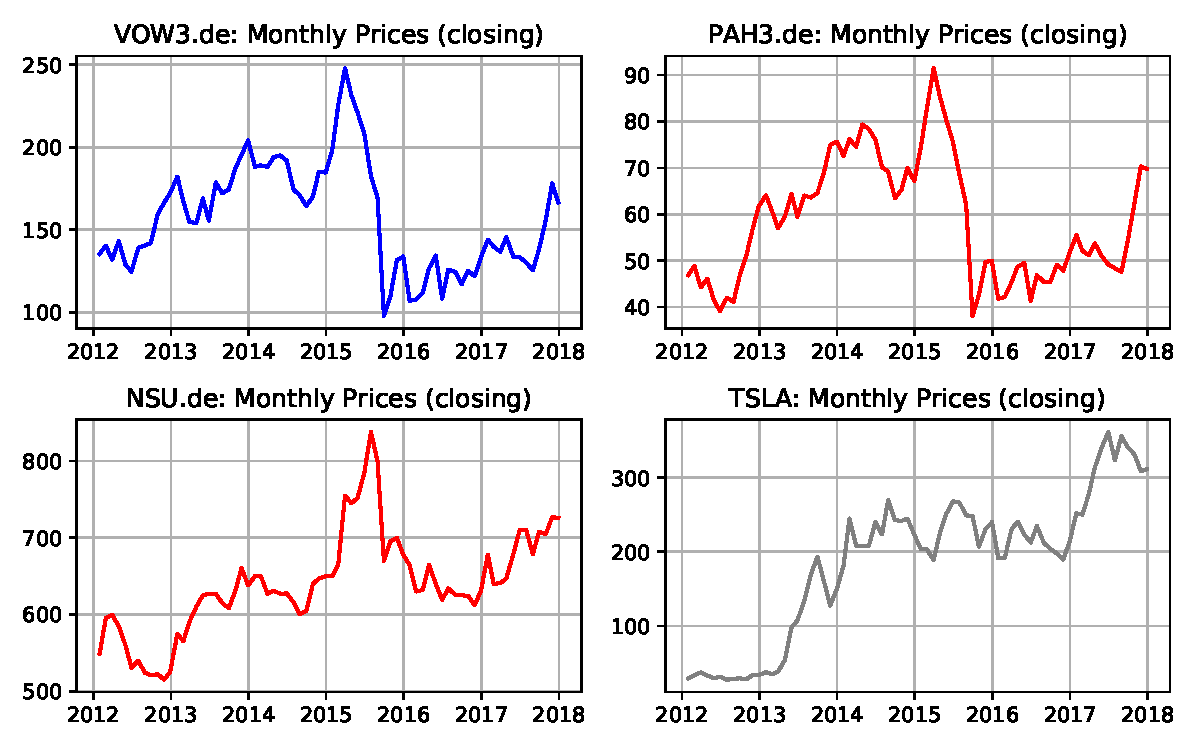
\includegraphics[width=\textwidth]{figures/intro/corr_prices.pdf}
%     \caption{Closing monthly stock prices for four corporations from the automotive industry (clockwise from top left): Volkswagen AG (VOW3.DE), Porsche Automobil Holding SE (PAH3.DE), Tesla, Inc. (TSLA), Audi AG (NSU.DE)}
%     \label{fig:stockprices}
% \end{figure}

% \todo{Find example with american companies}

% The case example for correlating stock prices in Figure~\ref{fig:stockprices} illustrates how the subsidiary corporations Porsche and Audi relate to their parent corporation VW. The huge drop in 2016 represents the emissions scandal which affected all three corporations. Especially the Porsche stock price moves very similar to the stock price of Volkswagen but also the Audi stock price shows some similarity. As an counter example the Tesla stock price is shown which does not reveal any deep relation with the other ones. This first analysis only gives a first insight into the potential relationships between stock corporations. As a part of this thesis I will investigate the dependency of these econometric time series using statistical tests like the Engle–Granger two-step method for testing cointegration between related stock prices.  \todo{Reformulate}

\section{Problem Definition}
\label{section:problem_definition}
A company's economical value needs to be assessed for use cases like asset investment, speculative trading of stocks, estimating a company's credit risk or making internal business decision in consideration of competitors, suppliers and business partners. In the context of market analysis and financial forecasts, the economical value of a stock is called the intrinsic value.

% Add to problem definition: The stock market is driven by events and emotions. It will be investigated if there are underlying structures between stock prices which can be observed by variables extracted from financial news and stock price.

As implied by the theory of Bounded Rationality, the intrinsic value of a company's stock is likely not fully reflected by its actual stock price. Business relationships are assumed to partially explain this gap between intrinsic and actual value of stock prices. Concluding, the goal of this work is to \textbf{improve the assessment of a company's intrinsic value by taking its business relationships into account}.

In contrast to their formal definition, this works treats business relationships in a wider context as from the perspective from a single company. Every negatively or positively connotated connections between two companies is considered as being part of their business relationship. Thus, a related company can be any type of company having an direct or indirect influence on the success or failure of another company's business. For example, one company can have an indirect impact on another one by being its competitor.

However, neither the intrinsic stock value nor the business relationships can be determined objectively by some measures. If a business relationship between two companies is present, both stock prices are assumed to evolve similarly. In order to evaluate the above suggested impact of underlying business relationships on a stock's intrinsic value, the impact on cross-correlations between two stock prices will be examined respectively. Subsequently, if two stock prices reveal a similar evolution, it is assumed to be, at least partially, caused by an underlying business relationship between the two affiliated companies.

Last but not least, a business relationship is an abstract property which encompasses a set of various uni- and bidirectional relations, as defined before. Due to their branched nature, the complex composition of relations is not directly observable, news are considered to be an appropriate proxy for this information. Furthermore, financial news in particular will be used because they are \enquote{deemed to have less noise compared with general news}, as stated by \citet{KhadjehNassirtoussi2014TextReview}. Hence, it is assumed that business journalists associate two companies with each other in their financial reporting if they are related in some sense.


% Eqn.~\ref{formula:hypothesis}:

% \begin{align}
%     \begin{split}\label{formula:hypothesis}
%         H_0 &= \text{There is no statistical significant correlation between stock price cross-correlations and business relationships} \\
%         H_1 &= \text{There is a statistical significant correlation between stock price cross-correlations and business relationships}
%     \end{split} \\ \eqname{Null and Alternative Hypothesis}
% \end{align}


% https://en.wikipedia.org/wiki/Fundamental_analysis

% "The paper is organized as follows. In sect. 2 we present our results for thermodynamic quantities. Correlation length measurements are presented and discussed in sect. 3. A summary is given in sect. 4."
% https://drive.google.com/file/d/1GMD2dBogilx3JVeUiRyek3yz8IlJ6C1g/view
% https://sci-hub.se/10.1080/14697688.2015.1070960
% https://sci-hub.se/10.1016/j.eswa.2014.07.040
% https://sci-hub.se/10.1016/j.eswa.2014.08.004

\section{Background}
\label{section:background}
The following subsection provides a brief introduction into the financial markets and how to treat economic variables. Consequentially, the next subsection covers statistical hypothesis test which will be used excessively in the later evaluation of stock prices in Section~\ref{subsection:time_series_evaluation}. However, it should be noted that financial theory, econometrics and statistics are broad fields for which a comprehensive introduction cannot be provided in this work.

\subsection{Stock Markets}

% Financial sector finances the real economy, i.e. companies with product-oriented business.
% e.g. Origins of Apple

% securities are bonds, stocks 

Capital markets are very important in modern economy. Because companies usually need money for productive use in advance, investors come into play giving the opportunities for companies to emerge and develop. For linking people who hold capital with those seeking capital, stock exchanges enable the fast capital flow among them. The traded capital on these exchanges defined by so called securities.

A security is a financial instrument which accommodates several categories in which one can invest. The most common type of securities are shares representing the investment in an entity like a company. An investor buying shares of a company thereby becomes a shareholder including the right to share in the company's profit and the right of co-decision in terms of corporate policy. The value of such shares is determined by the company's worth, which in turn is determined by supply and demand for its shares in the market. Besides these natural market dynamics, the price might also be affected by events like stock splits.

\paragraph{Stock Splits}
Such stock splits are adjustments to the number of available shares and their respective price. If the price increases substantially up to a high value, the shares becomes less affordable to small investors. Hence, the number of shares might be doubled and share prices halved in order to ensure the same amount of traded money for this company but also more affordable share prices. As an extreme example, the price for one share in \emph{Apple Inc.} almost reached \$700 in 2014. Subsequently, they issued a 7-for-1 stock split, which led to seven times shares as before, to make their shares more accessible to potential shareholders.

If investors are speaking of shares in multiple companies, these shares are called stocks which do not refer to a particular company. Throughout this work, the more general term stock is used, even though it might refer to a single company.
% https://www.stlouisfed.org/education/tools-for-enhancing-the-stock-market-game-invest-it-forward/episode-1-understanding-capital-markets 
% https://www.quora.com/How-exactly-do-stock-prices-get-determined
% https://www.investopedia.com/terms/c/capitalmarkets.asp
% https://www.investopedia.com/ask/answers/difference-between-shares-and-stocks/
% https://www.investopedia.com/terms/s/stocksplit.asp

\paragraph{Market Indices}
Because stock exchange tend to include an unmanageable number of shares, a stock market index is used which uses a selected number of stocks in order to represent the well-being of a separate sector of the market or even the whole market. Thereby, the index value is calculated by a weighted average of the share prices for these selected index components, whereas the weighting is usually based on the traded volume. For example, the \emph{NYSE Arca Oil Index} measures the performance of the oil industry by involving stocks of leading companies in this sector. To grasp the performance of the whole American stock market, a market index like S\&P~500 is proposed, which is an abbreviation for the rating agency \emph{Standard \& Poor's}. It includes 500 companies from two large stock exchanges, namely New York Stock Exchange (NYSE) and NASDAQ, whereby the number of index components might slightly diverge. Possible reasons for this are acquisition, merger, bankruptcy or dual-class listings. The latter one describes companies which provide multiple classes of stocks with varying voting rights for shareholders. To give an example, shares of \emph{Alphabet Inc.} are divided into three classes, where one class is reserved for founders and executives and therefore not publicly traded. It gives them ten times the voting rights as shares which can be bought by investors.

Besides market indices, another measure is quite common, namely the volatility. It seeks to capture the uncertainty of investors in the market by the stability of stock prices. A popular volatility index in the American stock market is the \emph{CBOE Volatility Index} (VIX) which measures volatility by the components of the S\&P~500 index. Hereby, one popular observation is a negative correlation between VIX and S\&P~500, i.e. the uncertainty increases if the market is performing poorly \cite{Fleming1995PredictingMeasure}.


\paragraph{Market Analysis}
Under the supposition of stock predictability, there are two common approaches for analysing and predicting market movements, namely \begin{enumerate*}[label=(\roman*)]
\item technical analysis and 
\item fundamental analysis
\end{enumerate*} \cite{KhadjehNassirtoussi2014TextReview}. The former one draws upon the belief that stock prices reveal patterns repeating themselves. Hence, historical stock prices are analysed in order to make predictions on their future movements. For analysis, the prices are typically represented by a multivariate time involving variables such as the high price, low price, opening price, closing price and trade volume. These five most popular variables are often referred to as OHLCV. Some popular analysis tools upon these OHLCV values are stock charts and technical indicators like moving average and momentum.

The second approach, fundamental analysis, considers a more sophisticated approach examining all available fundamental data that may influence market movements \cite{LopezdePrado2018AdvancesLearning}. Instead of using statistical methods on pure numerical data, company related information and external factors, such as corporate policy and the political climate, are included into the assessment of a company. A popular source for collecting information like these are financial news since they are known to influence financial markets \cite{Vlastakis2012InformationVolatility, KhadjehNassirtoussi2014TextReview}. Based on the comprehensive conduction of a company, its intrinsic value is approximated. If the current stock's price does not reflect the assessed value, a fundamental analysis recommends investing into this stock before it converges to this value in the future. This method is supported by research revealing that stock prices need some time to adapt to new information \cite{Hsu2016BridgingEconomists}.

% https://drive.google.com/file/d/18l7y9Oh9uEo6yANFsUDggIIaOPDYqsR1/view



% https://drive.google.com/file/d/1ToXIJMtIPe2d-rU1EqozIqP_pkZSrUv1/view
% https://drive.google.com/file/d/18l7y9Oh9uEo6yANFsUDggIIaOPDYqsR1/view
% https://sci-hub.se/10.1016/j.eswa.2014.07.040
% https://www.fundamentalsofaccounting.org/fundamental-technical-analysis/
% Short intro to Quantitative, Fundamental, Technical Analysis: Vargas2017

% \emph{The second or millisecond impact prediction is the element that fuels an entire industry by the name of micro-trading in which special equipment and vicinity to the news source as well as the market computer systems is critical} \cite{KhadjehNassirtoussi2014TextReview}

%  Hsu et al. (2016) points out, that stock prices do not reflect new information immediately, but need some time to adapt to it. Forecasting the markets behaviour over the next hour (Short-term) is therefore affected by higher volatility and lower predictive accuracy. Then again, the new information loses its advantageous influence usually over the next days except for extreme influences like the Lehman bankruptcy (Yoshihara et al. 2014). As a trade-off between these two boundaries, related work often focus on a prediction window of one day or week. When relying on information extracted from news, it is a common assumption that this information is of most value for the next days stock price movement. \todo{There should be many possible citations from the RW Statistics section}


% Side effects on the market:
% Examples for market manipulation like the Silver Thursday (Pincus and Kalman 2004)
% Mutual fund herding are not destabilizing but speeding up the price-adjustment to new information (Wermers 2002)
%  There are pattern like the Monday Effect or the January Effect and U shape in intraday volatility
% As stated in the previous section, investors are expected to act rational and therefore ensure a stock price which is close to its intrinsic value.



% Optional:
% Australian and New Zealand stock prices are unit root process denying their predictability. Evidence for EMH: \cite{Narayan2005} TODO: Evidence against EMH (Predictability is existing \cite{Hsu})
% The theory and hypotheses based on rationality originate from the Rational Choice Theory
% \emph{The literature of stock market prediction was initiated by economists (Keynes, 1937).} (Ding et al. 2014)
% On quantitative analysis and conclusion to ML: Tsantekidis2017


% Random Walk: "" (Regnault 1863)
% Became popular through the work by Malkiel1973 (A random walk down wall street)

% Efficient Market: "Theory of speculation" (Bachelier 1900)
% file:///C:/Users/Thomas/Downloads/Jovanovic_Le_Gall_2001.pdf
% file:///C:/Users/Thomas/Downloads/ObaladeandMuzindutsi.pdf

% Random Walk Theory states that stock price move accordingly to a random walk.
%  Three versions of the EMH are established: strong, semi-strong, weak. [...] In its weak form which is similar to the former random walk theory, the EMH states that price returns reveal a Brownian Motion, i.e. have no memory and are independent in time.
% https://www.researchgate.net/publication/284660721_Theory_of_speculation/citations

% Three forms:
% https://sci-hub.se/10.2307/2325486
% https://drive.google.com/file/d/1ToXIJMtIPe2d-rU1EqozIqP_pkZSrUv1/view
% Weak:
% https://investinganswers.com/financial-dictionary/economics/weak-form-efficiency-5172
% https://www.investopedia.com/terms/w/weakform.asp
% EMH vs RWT: https://quant.stackexchange.com/questions/25794/do-efficient-market-hypothesis-and-random-walk-theory-convey-the-same-concept/25796


% \subsection{Econometrics}
% https://www.researchgate.net/post/Any_recommended_techniques_for_testing_causal_relations

% \begin{itemize}
%     \item Order Of Integration / Unit root (-> econometric time series are considered to be unit root)
%     \item Most economic data is I(1), non-stationary (http://cmi.comesa.int/wp-content/uploads/2014/06/Stationarity-and-Cointegration-Analysis.pdf)
%     \item Cointegration and Error Correction Models (Engle and Granger’s two-step procedure)
%     \item Vector Autoregression
%     \item Granger Causality (vs. real causality)
    
%     \item Explain order of integration since its value is mandatory to know before looking out for features like cointegration, correlation or Granger Causality
% \end{itemize}


\subsection{Statistics}
\label{subsection:bg-statistics}

The science of statistics mainly deals with data-based methods. A substantial tool in order to describe data without any foreknowledge are data distributions on which further analysis and interpretation can be conducted. Among the manifold of data distribution, the most popular one is the normal (or Gaussian) distribution.
 
 % The family of Student's t distribution varying in kurtosis. The greater t gets, the more similar it becomes to to a normal distribution.

Since in many real-world cases the underlying data distribution is rather unknown, inferential statistics expect samples of a population to be representative for the regarding distribution of this population. The likeliness of observations based on such samples to be true for the whole population, increases with the number of samples which is described by the law of large numbers.

\paragraph{Skewness and Kurtosis}
Using inference, statistics like mean, standard deviation, skewness and kurtosis of a data distribution can be approximated. Hereby, skewness and kurtosis are describing the dispersion of data. To be more specific, the former one describes the asymmetry of the distribution. While a skewness of zero represents a symmetrical distribution with the same number of data points on both sides of the mean, a positive or negative skew indicates that the mass of the distribution is concentrated on the left or right side respectively, as seen from the mean. Kurtosis measures the thickness or heaviness of the tails of a distribution. High kurtosis (greater than three) describes a high peak in the center and heavy tails, which can also be seen as evidence for many outliers. Conversely, a distribution with low kurtosis has light tails and therefore appears to lack outliers. While a distribution with a kurtosis of three (as in the normal distribution) is called mesokurtic, it is called leptokurtic or platykurtic for a higher or lower value respectively. Financial variables often indicate a leptokurtic distribution leading to more extreme values or values closer to the mean \cite{Franke2010StatisticsMarkets}.


\paragraph{Hypothesis Test}
In quantitative research, hypothesis tests are examined on data samples in order to draw probabilistic conclusions. These conclusions can be generalized for the underlying population of the observed samples. Therefore, usually a null hypothesis $H_0$ and a contrary alternative hypothesis $H_1$ are defined. For example, the Jarque-Bera test \cite{Jarque1980EfficientResiduals} defines a null hypothesis that the investigated samples are drawn from a normal distribution. The resulting test statistic is usually transformed to a probability $p$ representing the probability of observing the selected set of samples, given the null hypothesis is true. Hence, $p$ can be used to reason about whether or not the collected data fits the previously defined hypothesis.

In order to decide if the null hypothesis can be rejected and therefore prefer the alternative hypothesis, a significance level $\alpha$, e,g, 0.05, is defined in advance which functions as a cut-off value. Choosing a smaller $\alpha$ suggests a more robust interpretation of the null

If $p \leq \alpha$, one found significant evidence in favour of $H_1$. Choosing a smaller $\alpha$ ensures a more robust outcome for this interpretation. Otherwise if $p > \alpha$, it is stated that the test failed to reject $H_0$. Though, one cannot accept $H_0$ by design of the test.

When conducting hypothesis tests in Section~\ref{subsection:time_series_evaluation}, multiple tests will be applied to ensure more stable results. However, the outcome of such hypothesis tests should be treated with caution. They only provide probabilistic results based on what is more likely to be true.

Most hypothesis tests rely on some statistical assumption on the samples used for testing. One important constraint is that samples are independently and identically distributed (i.i.d.). Hence, large samples drawn from the same population are expected to reveal approximately equal properties and therefore lead to the same results during inference. When it comes to time series analysis, there are some popular cases known for which samples are known to be not i.i.d.:
% \begin{enumerate}[
% leftmargin=0pt, itemindent=20pt,
% labelwidth=15pt, labelsep=5pt, listparindent=0.7cm,
% align=left, label=(\roman*)]
\begin{itemize}
    \item A non-stationarity variable involves samples depending on time and thus they are not identically distributed.
    \item If the samples of a variable are found to be autocorrelated with previous samples, they are not independently distributed.
    \item The variance of a time series, also denoted as volatility, might change over time. This is referred to as heteroscedasticity (heterogeneous volatility) and contradicts with being identically distributed because the variance is not stable.
\end{itemize}

To give an example in favour of i.i.d., a independent white noise process fulfills all constraints. It requires \begin{enumerate*}[label=(\roman*)]
    \item to have no autocorrelation (serially uncorrelated)
    \item zero mean,
    \item constant and finite variance and
    \item independently drawn samples
\end{enumerate*}. The correlation measure Pearson's $r$ which is used throughout this work, assumes samples to be i.i.d. Hence, it need to be examined if any contradictions exist.

%  are an important assumption in many inferential statistics like Pearson's $r$ which uses samples to approximate the correlation of their regarding populations. Further, the population is required to be normal distributed but studies showed that it is quite robust for non-normal distributions \cite{Bishara2012TestingApproaches}.
% https://sci-hub.se/10.2466/pms.1976.43.3f.1319
% If two variables are i.i.d., then they must have the same distribution.Which means they have the same parameters namely mean, std dev.
% 3. iid is more precisely defined concept. If e.g. stock returns are iid, it means they are drawn from the same distribution each day. If people say that something is random, they usually mean unpredictable. For example if stock returns are drawn some days from distribution with high variance, and other day from distribution with low variance, they are still random (not predictable), but they are not iid.



% Sources:
% https://statistics.laerd.com/statistical-guides/hypothesis-testing-2.php
% https://machinelearningmastery.com/statistical-hypothesis-tests/
% https://stattrek.com/hypothesis-test/hypothesis-testing.aspx
% https://www.researchgate.net/post/1_What_is_the_relationship_among_iid_randomness_autocorrelation_heteroskedasticity
% https://math.stackexchange.com/questions/223373/iid-variables-do-they-need-to-have-the-same-mean-and-variance

% Optional:
% The area below $\alpha$ is called the region of rejection and 
% is called the confidence interval or region of acceptance which 

% one or two-tailed statistic
% type I and type II errors
% instead of p, sometimes only the test statistic is given. For those cases, critical values (which are usually provided within tables) can be used which denote the appropriate values for common significance levels, such as 0.10, 0.05 or 0.01.

% For example, the significance for an observed correlation statistic can be determined by transforming it to the confidence intervals of a hypothesis test 


% e statistical inference procedures designed to test that the underlying distribution of a random variable is normally distributed

\section{Methodology}
\label{section:methodology}
In order to investigate the impact of business relationships on the correlation of stocks, features need to be extracted at first. In the following, the methods used for feature extraction and evaluation will be presented.

\paragraph{Stock Correlation}
For measuring the correlation among two stocks, the correlation coefficient among their historical prices over a period of four years will be calculated. Because economic variables, and thus stock prices, are considered to be unit root processes \cite{Granger1974SpuriousEconometrics}, they are very likely to falsely reveal mutual correlation, also known as spurious correlation. Regressing on such variables therefore leads to spurious regression \cite{Yule1926WhyTime-Series}. To filter out potential causes for this error, the data needs to be prewhitened \cite{Dean2016DangersModels} and statistical conditions for correlation and regression need to be assured. According to \citet{Granger1974SpuriousEconometrics}, one should not expect the data to be completely free from spurious correlations, even though the aforementioned step were applied: \enquote{Although any of these methods will undoubtedly alleviate the problem in general, it is doubtful if they will completely remove it}. Because a large set of stock prices will be used throughout this work, the results cannot be individually checked or visually evaluated. Instead, a diverse set of hypothesis tests will be applied to find evidence for statistical properties like stationarity. After reducing potential causes for spurious correlation and thereby ensuring preconditions for correlation testing, the Pearson product-moment correlation coefficient, denoted as $r$, will be calculated.

\paragraph{Co-occurrence}
Besides the stock correlations, a second feature needs to be introduced which represents the business relationship. As stated previously in Section~\ref{section:problem_definition}, financial news are used therefore. They are known to be strongly linked to the market in both directions, i.e. they not only report market status but they actively create an impact on investors behaviour \cite{KhadjehNassirtoussi2014TextReview}. Hence, they are considered to be an appropriate source of information for finding business relationships. Thereby, the simultaneous occurrence of two companies in an article is considered to be representative for their relationship. The joint appearance will be called co-occurrence in the following. In order to identify occurrences of companies, Named Entity Recognition (NER) will be applied. NER is a method of information extraction which locates sequences of words in an unstructured text and labels them by predefined general categories, such as \enquote{person}, \enquote{location} or \enquote{organization}. To filter and link found organization entities to historical prices, Named Entity Linking (NEL) will be used, which seeks to link classified entities to entries from a selected knowledge base. The used knowledge base will contain historical stock prices, ticker symbols (e.g. \emph{MSFT}) and official company names (e.g. \emph{Microsoft Corp.}) which can be used for NEL. Based on the extracted and linked occurrences, three handcrafted features with differing emphasis on either frequency or distance of co-occurrences will be introduced in Section~\ref{section:text_analysis}.

\paragraph{Evaluation}
In order to assess the success of feature extraction and to evaluate my hypothesis, the correlation between the two extracted features stock correlation and co-occurrence is calculated and discussed. To compare the three co-occurrence based features with each other, they will be correlated separately with the stock correlation feature. The most meaningful feature is expected to reveal the highest correlation. Subsequently, the most promising news-based feature resulting from this experiment is used to retrospectively assess the prewhitening steps for stock prices. The stock correlation will be calculated for every intermediate preprocessing step in order to evaluate if they are supportive for a higher correlation with co-occurrence. Finally, my hypothesis is evaluated by the overall observed correlation coefficients between both resulting features, extracted from stock prices and financial news. To ensure the coefficients significance, the confidence intervals will be provided.

% Any attempt to evaluate the results would be premature at this stage, since some of these initiatives require more time for concrete and tangible results to be reached.  % http://www.forschungsgesellschaft.at/rereal/TOWARDS%20A%20FRAMEWORK%20IN%20OFL.PDF

\paragraph{Limitations}
The financial markets are prone to a vast number of external influences which cannot be all collected. Especially, political tension and other events can have a huge impact but are not easy collectible because they might be missing in financial reporting. Further, financial markets across the world reveal different dynamics \cite{Hsu2016BridgingEconomists} and need to be examined separately with suitable data. For those reasons, some problem limitations are defined in the following: 

\begin{itemize}
    \item Only the New York Stock Exchange (NYSE) and the NASDAQ Exchange will be considered. Measured upon market capitalization and number of listed companies, NYSE and NASDAQ are the world's largest exchanges. Consequently, findings based on these might be supported for other great stock exchanges, such as Tokyo Stock Exchange and Shanghai Stock Exchange, but need to be examined by an appropriate dataset.
    \item Both exchanges contain more than 3000 companies each. Because small companies are less likely to be mentioned in financial news, only components from the S\&P~500 market index are used which are considered to be the most important ones for the two exchanges.
    \item Business relations are not steady, but fluctuate and vanish and new ones emerge due to an altering corporate policy. This problem is not treated and the relationships are considered to be steady for the examined period. Subsequently, the stock correlations and news-based co-occurrences for the whole period are collected, each one condensed to one coefficient per pair of companies.
\end{itemize}

In practice investment corporations are optimizing their prediction models with every bit of information which might be useful. The markets behavior will always adapt to new trading algorithms and thereby its market efficiency vanishes such improvements. Hence, investors try to keep their intellectual capital saved and usually do not share successful autonomous trading methods - to the chagrin of the scientific community. Therefore, it is challenging for scientists to develop a system which accommodates real-world constraints \cite{Vanstone2009AnNetworks}. Also, a high degree of random factors remains, among others, because of the offer-demand-fluctuations. With obstacles as the previously mentioned ones in mind, this work does not aim for a proof of the hypothesis that business relationship are reflected in stock prices. Rather, evidence is collected in order to provide a potentially new direction of interest for research in market analysis and stock price prediction.

% \item Trading companies usually apply fast simple models for short-term predictions
% \emph{Given that the structure of an econometric model consists of optimal decision rules of economic agents, and that optimal decision rules vary systematically with changes in the structure of series relevant to the decision maker, it follows that any change in policy will systematically alter the structure of econometric models. (Lucas Critique, Philipps Curve)}
% \todo{Mention Lucas Critique}


% Let $t-1$ be the last day and $t$ be the first day in the future, the initial models input should be the historical stock prices of the target corporation over the last $D_P$ days $\{t-D_P, ..., t-1\}$. The stock prices for day $t$ are represented by opening price $p_{open}(t)$, day high $p_{high}(t)$, day low $p_{low}(t)$ and closing price $p_{close}(t)$. The model should then predict the direction towards which the price will change over the next $D_F$ days $\{t, ..., t+D_F-1\}$.

% As pointed out by \citet{Tsantekidis2017UsingMarkets}, only two classes $up$ and $down$ would introduce noise to the prediction labels, since the smallest changes would be considered as a upward or downward movement. To handle these cases a third class $still$ is introduced which represents no movement over the next $D_F$ days. A threshold $\epsilon$ will be defined which determines the margins of this third class. The label $y_t$ is then defined as follows:
% \begin{equation}
% 	y_t = \begin{cases}
%         1, & \text{if } p_{close}(t+D_F-1) > p_{open}(t) \cdot (1 + \epsilon) \\
%         -1,& \text{if } p_{close}(t+D_F-1) < p_{open}(t) \cdot (1 - \epsilon) \\
%         0, & \text{otherwise}
%     \end{cases}
% \end{equation}

% Based on this initial setup the model will be enhanced step by step with fundamental data of the target and its related corporations, the historical price of related corporations and their relationships to the target corporation. This graph data might be fed into the model as a matrix of feature vectors representing the graphs edges (corporate relationships), another matrix of feature vectors representing the nodes (general information, e.g. annual sales) and a third matrix for the historical stock prices of all considered corporations.

% The challenge of this work will be to generate an appropriate corporate network and build a prediction model exploiting this knowledge. Similar data is used as starting point as in the related work. The main emphasis is on transforming the raw text data into a reasonable structure format instead of introducing a better DNN for automatically extracting more meaningful relations.

\section{Related Work}
\label{section:related_work}
% Change focus: How to process stock prices. How to correlate them. Prediction only as information source
% Dont change too much but update the overall structure

% Feedback:
% review paragraphs - is it too big compared to its importance
% Break down approaches if not that related
% classify if approaches are necessary/important
% would a table help the thesis structure?


In the research area of modelling economic variables a plethora of approaches have been proposed, utilizing econometrics, Natural Language Processing (NLP) and machine learning. Predicting a stock's future behaviour is among the main research topics. Due to its practical application and its erroneous promise of easily earned riches, it received great attention. But the stock price prediction is a controversial topic and lacks a good theoretical foundation which justifies the approach of forecasts on finance markets. By ignoring these issues and applying machine learning approaches in sandbox like environments, some studies do not fully reflect the problem space and therefore erroneously promise investors easily earned riches. Consequently, the following related work is selected in terms of theoretical background required for understanding stock prices in general and promising prediction models on similar data. For a more comprehensive review of related work, I recommend the work by \citet{Hsu2016BridgingEconomists, KhadjehNassirtoussi2014TextReview, Cavalcante2016ComputationalDirections}.


A major issue in the related work of financial predictions is the comparability of results. There are a lot of different evaluation techniques like error rate \cite{Peng2016LeverageNetworks, Yoshihara2014PredictingNetworks}, Root Mean Squared Error \cite{Feuerriegel2018Long-termDisclosures}, Mean Absolute Percentage Error \cite{Bollen2011TwitterMarket, Xiong2015DeepTrends}, Theil’s inequality coefficient \cite{Bao2017AMemory.}, Cohen's kappa \cite{Tsantekidis2017UsingMarkets}, Area Under Curve \cite{Ballings2015EvaluatingPrediction} and Matthews Correlation Coefficient (MCC) \cite{Ding2014UsingInvestigation}. Some studies do not report an established data prediction metric at all, but instead test their model integrated in a trading strategy \cite{Deng2017DeepTrading, Ruiz2012CorrelatingActivity}. Of course, the real-world application is of high interest and should be tackled in the evaluation, but in addition, one should report some basic metrics. Consequentially, many scientists evaluate their performance in comparison to the probability by chance \cite{KhadjehNassirtoussi2014TextReview}. Another issue is the selection of the financial market since its maturity has a significant effect on the markets predictability \cite{Hsu2016BridgingEconomists}. For those reasons, the related work is not compared by their reported evaluation metrics but evidence is collected, on how to improve text-based stock price predictions in general.

With the high demand for good prediction models a vast number of data is available to researches. On the one hand, some studies focus on predicting the trend of stock prices via technical indicators like Bollinger Bands, momentum or Moving Average Convergence Divergence (MACD) \cite{Lee2014OnPrediction, Li2014NewsAnalysis, Yoshihara2014PredictingNetworks, Akita2016DeepInformation}, Bao et al. (2017), Patel et al. (2015). On the other hand, the whole market behaviour is predicted by the stock index or the volatility index \cite{Yang2002SupportPrediction, Bollen2011TwitterMarket, Zhang2011PredictingFear, Ding2014UsingInvestigation, Xiong2015DeepTrends}. Because the correlation of stock prices will be investigated, this work focuses on separate stocks instead of technical indicators or market indices. Still, these studies are of interest because they have to tackle similar problems caused by the noisy and stochastic nature of stock markets. 

% The overall field of market analysis is a very interdisciplinary one for which various research directions might be of interest.
The following approaches are splitted into two subsection. Because correlating stock prices requires conducting an intensive regression analysis, the following subsection particularly focuses on the predictability of time series in the context of econometrics and statistics. Methods like cross-correlation, mutual information and Granger Causality are proposed to measure and compare financial time series. Even though econometrics appear to be a hot topic in modern society, some fundamental knowledge of this research area is more than a century old and gives insights on how to set up meaningful similarity measures and models for noisy economic time series. Subsequently, the second subsection covers mixed prediction models for stock prices incorporating external information sources. Latest approaches benefit from the availability of data and computational power and therefore are better able to incorporate unstructured data like news and social media. To tackle the big amount of unstructured data, established methods from natural language processing and machine learning are applied.

\subsection{Statistical Analysis}

% \todo{Add Mantegna arguing for cross-dependencies in stock prices}
% Mantegna recalls the basic assumption of portfolio selection theory that there exists some kind of cross-dependencies between different stock prices.
% \emph{The stock market is far more complex than a collection of several independent random walks} (Mantegna)
% correlated, uncorrelated or weakly anti-correlated between pairs of stock prices on the NYSE (Mantegna)  \cit€{R.N.MANTEGNACross-correlationMarkets}

The predictability of the stock market is a highly competitive research area for which a great diversity of approaches have been proposed. On the one hand, scientists with economical or statistical background investigate the characteristics and quality of economic variables. On the other hand, scientists from the field of machine learning describe and evaluate new data-driven prediction models, often without tackling the systematic errors present in raw economic data. That is because machine learning models are supposed to learn relevant relationships and adapt their weights to the underlying probability distributions of the features. Bad or good prediction results are mostly used as arguments for the predictive performance of a model. Yet, the selection of the dataset itself might play a crucial role in the feasibility of a classification or regression problem. For example, \citet{Sun2016TradePrediction} report 70~\% accuracy for their matrix factorization model during training but only 51~\% on test data which is not a significant improvement compared to random guessing. On the contrary, \citet{Lee2014OnPrediction} present a Random Forest Classifier for predicting separate stock prices with an accuracy 22.2~\% higher than random guessing. Although results like these sound promising, it could be the consequence of an unsafe evaluation. Among various factors influencing an experiments outcome, models without cross-validation are prone to the \enquote{lucky sample effect}, as demonstrated by \citet{Hsu2016BridgingEconomists}. The time series might be lacking ergodic properties and therefore report erroneously high accuracy.

Further, \citet{Hsu2016BridgingEconomists} examine the crossfertilization between machine learning and econometrics in detail by shedding light on the applicability of the EMH and the disagreement between machine learning and financial economics literature. They collect and test several hypotheses concluding with some interesting findings: \begin{enumerate*}[label=(\roman*)] \item Technical indicators do not add a significant improvement to predictions;
\item SVM outperforms ANNs by a large difference;
\item machine learning approaches outperform econometric models (e.g. autoregression).
\end{enumerate*}

\citet{Kim2016AModel} applies a rule-based classifier on stocks from the energy sector of the US stock market. He calculates the cross-correlation among pairs of stocks and predicts a stocks price direction by considering the lagged stock price of another highly cross-correlated stock. For selected pairs of stocks they report an accuracy of 87.2~\% in average. Even though they select only highly cross-correlating pairs, potential spurious correlation are not considered which might arise due to unfiltered autocorrelations. As already pointed out by \citet{Granger1974SpuriousEconometrics} several decades ago, mis-specifications like omitted variables, irrelevant variables included or autocorrelations can lead to spurious correlation/regression. Therefore, instantaneously observed correlations might diminish over time.

\citet{Ruiz2012CorrelatingActivity} exploit these auto-dependencies of stock prices by training Auto Regression and Vector Auto Regression models with the Ordinary Least Squares (OLS) method to predict the final price on each day in the context of a regression task. Their approach combines stock price data with numerical features extracted from Twitter posts, e .g. the number of forwardings for a post.  Unfortunately, they do not inspect their data for homoscedasticity which is one of the requirements of the Gauss-Markov theorem for OLS to be the best linear unbiased estimator \cite{Hallin2014Gauss-MarkovStatistics}. Furthermore, they do not report statistical measures which can be compared to other work, but test their approach in a daily trading simulation ending up with 0.32~\% gain for the best model.

Instead of proving the predictability of a new introduced features by feeding it into a prediction model, \citet{Vlastakis2012InformationVolatility} apply a regression analysis between the demand for market-related information and market variables like volatility and stock prices. The overall information demand is represented by Google's Search Volume Index for the search keyword S\&P 500. The analysis includes hypothesis tests for Pearson's $r$ and uni- or bidirectional Granger Causality between the selected variables. In conclusion, they show that these relationship exists with a high certainty.

\citet{Kosapattarapim2017GrangerThailand} presents a very detailed procedure on inspecting Granger Causality between the stock exchange index of Thailand and the exchange rate between Thai Baht against US dollars. To ensure unit root time series and a cointegration relationship at a 5~\% significance level, they apply the Augmented Dickey-Fuller (ADF) \cite{Dickey1976IntroductionSeries} and the Johansen test. Both properties are mandatory before one can look for actual Granger Causality. Their results indicate an unidirectional causality from stock prices to exchange rate.

Besides univariate linear measures like autocorrelation and volatility another nonlinear property of time-series is the complexity/regularity which can be measured by approximate or sample entropy. The common Shannon entropy is not applicable since stock prices are considered to be non-stationary time-series. Therefore, \citet{Pincus2004IrregularitySeries} apply the approximate entropy on stock prices to measure a system's stability or irregularity. They conclude that this irregularity is a complementary property to volatility which is paramount for meaningful financial data analysis.

For a more conscious inspection of nonlinear auto-dependencies in finance time series, \citet{Dionisio2004MutualSeries} compare the normalized mutual information with Pearson's $r$ for several stock price indices. Referring to related work, they recall the assumption of a strong relationship between entropy, dependence and predictability. To exclude the linear auto-dependencies, they filter the data by taking the residuals of an autoregressive–moving-average process. Unlike the linear correlation, mutual information still indicates a significant dependency on the residuals without any foreknowledge on the theoretical probability distribution or the type of dependency.

% Detrended Cross-Correlation, Transfer Entropy, Sample Entropy between stock markets (2013)
% https://link.springer.com/article/10.1007/s11071-012-0680-z

% No Contagion, Only Interdependence: Measuring Stock Market Co-Movements (Forbes and Rigoborn, 1999)
% https://www.nber.org/papers/w7267.pdf


\subsection{Prediction Models}

Though this work is not focussing on predicting stock prices, the related work in this research area reveal relevant insights on the data and feature extraction. 

In the last decades the study of predictability on the stock market was a very popular topic for scientists. Especially the rapid achievements in predicting stock prices by applying models from the area of representation learning attracted attention. The first application of Neural Networks (NN) 30 years ago initiated a run on applying NNs and other related models. Before this time there were already other learning algorithms present like Linear Regression (LR), Support Vector Machines (SVM) and Genetic Algorithms. Usually, approaches based on NNs outperformed those other existing techniques partly by far \cite{Hsu2016BridgingEconomists, Yoo2005MachineEvaluation}.

To come up with valuable input for prediction models, the unstructured data needs to be preprocessed. This process has a significant impact on the success of the prediction models and therefore requires sophisticated approaches. \citet{KhadjehNassirtoussi2014TextReview} provide a broad overview of related work based on these three aspects and review in terms of feature-selection, dimensionality-reduction and feature-representation.

% For instance, \citet{Tsantekidis2017UsingMarkets} apply a LSTM on Limit Order Books containing all buy and sell orders of a stock for prediction a stock prices movement. 
% One of the first NLP approaches on price prediction: https://www.researchgate.net/publication/3776378_Daily_stock_market_forecast_from_textual_web_data



% \suggest{To tackle the big datasets deep learning technique are applied as an improvement of previous NNs. As pointed out by \citet{Chong2017DeepStudies} deep neural networks (DNN) are able to extract abstract features from a large dataset without any prior knowledge of predictors.}{}
Since external information related to stock markets is not directly observable, meaningful proxies are extracted from unstructured data like forum posts, news, social media and SEC filings. The most popular text sources are financial news \cite{Peng2016LeverageNetworks, KhadjehNassirtoussi2015TextSentiment, Zhai2007CombiningPrediction} because they are expected to represent new events influencing the financial market. Their importance is mostly reflected within the stock prices of the directly following days and loses its meaning over a longer time period \cite{Ding2014UsingInvestigation}. Therefore, many scientists incorporate news for short-time prediction models \cite{KhadjehNassirtoussi2014TextReview}. They consider the news and the previous daily stock prices to predict the intraday price movement for the next day. The market return for this relatively short time span is known as \enquote{open-to-close}. Various methods for extracting abstract representations of news have been proposed over the last years. Most of the following presented approaches can be counted to deep learning since they rely on big datasets and learn abstract hierarchical representations by applying two or more hidden layers in their networks.

\citet{Ding2014UsingInvestigation} compares linear and nonlinear approaches for prediction using events-based document representations without incorporating historical stock price data. They extract events by applying Open Information Extraction (OIE) on news articles from \textit{Reuters} and \textit{Bloomberg}. Thereby each article is transformed into a tuple of subject, predicate verb and object. The applied DNN achieves 60~\% accuracy for predictions of the S\&P 500 index. For the prediction of individual stocks it even surpasses 70~\% accuracy, even though they do not consider the stock price of the previous days at all. One main finding of their work is the advantage of less but more qualitative data (news titles) in contrast to much noisy text data (whole article contents). This indicates that thoughtful preprocessing is a very import task for text-based approaches. \citet{Zhai2007CombiningPrediction} suggests a SVM for combining textual and numerical data. News texts from \textit{The Australian Financial Review} are accumulated by a semantic network called WordNet. It creates 30-dimensional semantic representation of an article's content. Compared with their own single source systems, results of 70~\% accuracy indicate that news combined with technical indicators can improve the predictability of a stock's daily movements. Since there are events on the finance market whose impact do not fade out within days but weeks or months, \citet{Yoshihara2014PredictingNetworks} sheds light on a novel deep network for incorporating events with longer-term impacts. They enhance a Recurrent Neural Networks-Restricted Boltzmann Machine (RNN-RBM) with a Deep Belief Network (DBN) and apply it for prediction of Nikkei stock price movements on the next day. However the results are not tremendously above their heuristic baseline (about 3~\% improvement), indicating that their approach only adds a slight improvement. Hence, their model might lack some contextual information since it only relies on the news articles collected from \textit{Nikkei Newspaper}, not considering the previous behaviour of the related stock price.

Previous work usually only considers one company for predicting its future stock price as pointed out by \citet{Akita2016DeepInformation}. Instead, they feed related articles and historical prices of ten companies within the same industry at once into a LSTM to predict the close prices of all ten companies by regression analysis. \textit{Nikkei newspapers} are preprocessed using Paragraph Vectors which learns fixed-length feature vectors from variable-length texts. Their market simulation indicates that incorporating multiple companies from the same industry is very effective for stock price prediction. Unfortunately, a comparable evaluation using metrics like accuracy is missing.

A recent approach by \citet{Chen2018IncorporatingPrediction} explores the setup and application of a corporation graph for a prediction model. Due to its relevance this approach will be examined more detailed as the previous ones. A graph is proposed which contains nodes representing stock companies from Shanghai Stock Exchange and Shenzhen Stock Exchange and their shareholders. The weighted edges between those nodes indicate the shareholding ratio. Based on this graph two approaches are presented for incorporating the data into a NN: The first one maps each company node into a vector using various node embedding techniques. For predicting a company's stock price movement the ten closest nodes are selected, the related historical prices accumulated into a vector and fed into a LSTM-Encoder. Based on the outcome of this layer they apply a binary classification layer which should output if the stock price will rise or fall on the next day (open-to-close intraday movement). The second more advanced approach tackles the issue of summarizing all the information and not considering each relation separately. Therefore, they apply a joint model based on a Graph Convolutional Network (GCN) which incorporates the whole network. A combination of a LSTM baseline and their GCN model yields the best results. While the baseline obtains an accuracy of about 53~\% the graph based enhancement improves it by almost 5~\%. 

Both of the introduced approaches sound promising for investigating them closer in my work.
The latter work can be seen as a proof of concept. Considering relations among companies can improve the predictability of a stocks behaviour. However, they select companies by their similarity since their graph's edges only represent share ownerships. For the well-being of a company, and therefore also of its stock, the performance of cooperating companies is crucial. If a supplying or subsidiary company is not doing well, the graph should reflect which companies might be infected by this one. Therefore, it is suggested to extract representative features of business relations among companies like the same industry, subsidiaries, co-operations and supplies.

% % quote from the booktabs documentation: 1. Never, ever use vertical lines. 2. Never use double lines. I tend to agree

% Categorical (vs. Regression)
% Multiple Companies
% Unstructured (Text Based)
% Fundamental and/or Technical Analysis
% Stock Price Related (vs Index/Indicator)
% Long vs. Mid vs. Short Term
% Stock Exchange / Index / Company

\newcommand{\mlcell}[2][c]{%
  \begin{tabular}[#1]{@{}c@{}}#2\end{tabular}}

\begin{table*}[!ht]
    \centering
    \setlength{\tabcolsep}{0pt} % Default value: 6pt
    {\tiny
    \begin{tabular*}{\textwidth}{@{\extracolsep{\fill}}cccccc} \toprule
        {Authors (year)} & {Data source} & {Target output} & {\mlcell{Sampling\\period}} & {Method} & {\mlcell{Performance\\measure}} \\
        \midrule \mlcell{Ding et al.\\(2014)} & \mlcell{Reuters \& \\Bloomberg} & \mlcell{up/down over\\days/weeks/months} & 2006-2013 & OIE & MCC \\
        \smallskip \\
        \mlcell{Zhai et al.\\(2007)} & \mlcell{Australian Financial\\ Review (1 comp.)} & \mlcell{up/down over\\ the next day} & 2005-2006 & SVM & acc. \\
        \smallskip \\
        \mlcell{Yoshihara et al.\\(2014)} & \mlcell{Nikkei Index \&\\Newspaper} & \mlcell{up/down of\\next days MACD} & 1999-2008 & RNN+RBM+DBN & error rate \\
        \smallskip \\
        \mlcell{Akita et al.\\(2016)} & \mlcell{Nikkei 225 comps. \&\\Newspaper} & \mlcell{regression of\\close price} & 2001-2008 & \mlcell{Paragraph Vector \&\\LSTM} & \mlcell{market\\simulation} \\
        \smallskip \\
        \mlcell{Chen and Wei\\(2018)} & TuShare - SSE \& SZSE & \mlcell{up/down over\\ the next day} & 2017 & LSTM \& GCN & acc. \\
        \bottomrule
    \end{tabular*}}
    \caption{A summary of related studies on stock market prediction.}
    \label{table:research_overview}
\end{table*}
% \todo{Deprecated from expose}
% For a quick overview Table~\ref{table:research_overview} provides a summary of the following presented recent work.


% Authors (year)

% Features (e.g. Technical Indicators, Historic Closing Stock Prices, Historic OHLCV, Word Vector, Sentiment Vector, Bag of Words/Keywords, Fundamental Var.)
% Prediction Model / Method (e.g. ANN, LSTM, RL, VAR, Cross-Correlation, SVM, LR, SOFNN, DBN)
% Predicted Variable (Regression, Binary, 3 Classes, Other (e.g. 5 classes))
%? Prediction Window (Short-/Mid-/Long-Term)
% Performance measure (e.g. MSE/RMSE, Cohens Kappa, F-Score, Accuracy, Return of Invest)

% Data source (provider)
% Type of data (Stock Price, Finance News, Stock Index, US-Dollar-Index, Tweets Sentiment, Limit Order Books)
% Amount of Samples (train/val/test?)
% Market / Stock Exchange (e.g. Bombay Exchange, NYSE, NASDAQ, SSZE)
% Sampling period (covered years)

\section{Data}
\label{section:data}
\subsection{Financial News}
For extracting features describing the relationship among companies, financial news are chosen to be a good source of information. Most of the reviewed related work relies on news articles since its impact on the financial markets is a common presumption in the literature \cite{KhadjehNassirtoussi2014TextReview}. For this study, a dataset will be used consisting of financial news \footnote{https://drive.google.com/drive/folders/0B3C8GEFwm08QY3AySmE2Z1daaUE} released by \citet{Ding2014UsingInvestigation}. It contains news articles from Reuters \footnote{https://www.reuters.com} (106,519 documents) and Bloomberg \footnote{https://www.bloomberg.com} (448,395 documents) covering the time period from 2006-10-20 to 2013-11-26. Those texts will be used for extracting features like co-occurrences. How to extract these features and evaluate their informative value will be tackled in Section~\ref{section:text_analysis}.

Since this feature extraction will heavily rely on the content within articles, duplicated articles, empty articles and articles with a content length less than 300 characters will be removed.

\begin{figure}[!ht]
    \centering
    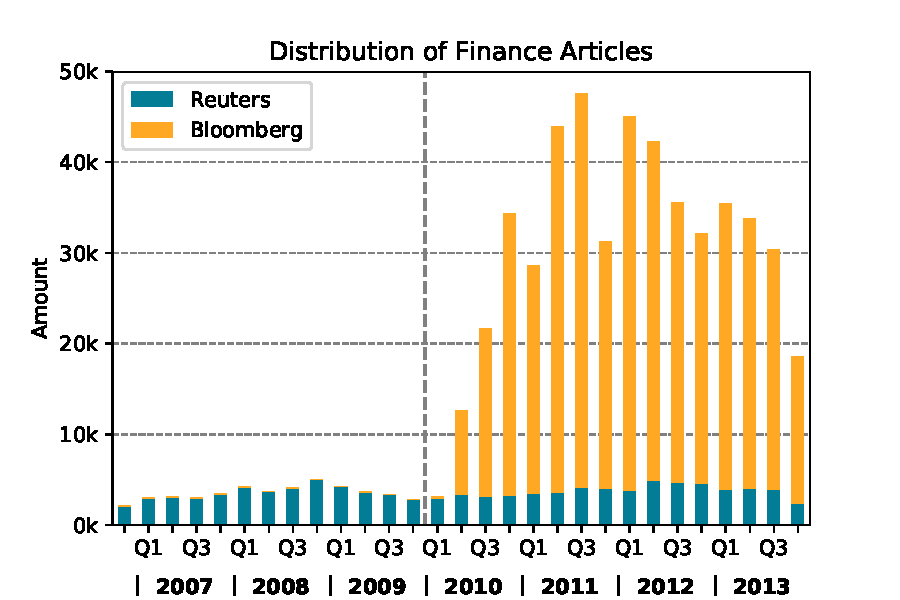
\includegraphics[width=0.8\textwidth]{figures/data/articles-distribution.pdf}
    \caption{Distribution in time for all articles after dropping empty, meaningless or duplicated ones. The dashed vertical line marks the beginning of the stock price dataset, introduced in the next step.}
    \label{fig:articles-distribution}
\end{figure}

After the most problematic properties of the data are tackled, there are 542,517 articles left. Figure~\ref{fig:articles-distribution} shows the distribution of these articles over time. While Reuters articles are equally distributed over all covered years, most of the Bloomberg articles are from 2010 until 2013.


\subsection{Stock Prices}
Stock prices are collected from a published dataset containing the historical prices for all components of the stock market index S\&P 500 from 2010 to the end 2016 \footnote{https://www.kaggle.com/dgawlik/nyse}. For each stock the daily open, high, low, close and volume values (OHLCV) are given in US dollar. The dataset already accounts for stock splits (Section~\ref{section:background}) by adjusting prices to the end of the time period. Thus, price values of affected stocks in 2010 are rectified to have the same meaning as in 2016.

For linking stock prices with occurrences in the previously introduced news dataset, we will be using the company names in the securities table from the same published dataset.

Since there are no financial news available after 2013-11-29, the stock prices after this week are discarded. However, the financial news before 2010 will be used, even though no stock prices are collected for this time period. The relational features which will be extracted are assumed to have a long-term impact, so it will be evaluated in Section~\ref{section:evaluation}, if incorporating information from news between 2006 and 2010 is helpful.

\begin{figure}[!ht]
    \centering
    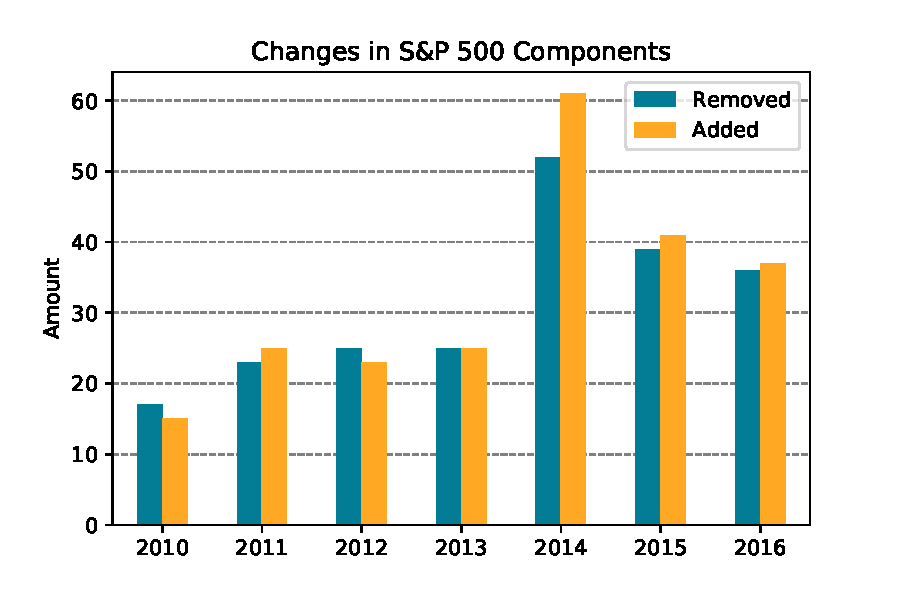
\includegraphics[width=0.8\textwidth]{figures/data/sp500-comp-changes.pdf}
    \caption{Starting with 499 components in 2010, the index underwent 217 removals and 227 additions until the end of 2016. The historical components for the S\&P 500 index were collected from an anonymous distribution page. \protect\footnotemark}
    \label{fig:sp500_changes}
\end{figure}

\footnotetext{https://nemozny.github.io/datasets/}

The selected stock price dataset accounts only for companies present in the S\&P 500 index at the end of 2016. As shown in Figure~\ref{fig:sp500_changes}, the index' components are continuously changing due to various reasons like acquisition, merger, dual-class listing or bankruptcy. Because we only have the prices for components from 2016, we ignore that some companies we are looking at are not actually part of the index during the observed time period. To avoid incomplete time series, stocks which were not continuously present are left out. In addition to the stock prices, overall measurements of the performance and the confidence at the NYSE for the same period as the stock prices need to be considered. Being popular variables for this purpose, the CBOE Volatility Index (VIX) \footnote{https://www.kaggle.com/lp187q/vix-index-until-jan-202018} and the S\&P 500 index (GSPC) \footnote{https://www.kaggle.com/benjibb/sp500-since-1950} are selected. As already observed by \citet{Fleming1995PredictingMeasure} when the VIX was introduced, there appears to be a strong negative relationship between volatility and stock market returns. Indicators supporting this assumption, can be seen in Figure~\ref{fig:index_and_vix} showing the closing values for both variables over the observed period. The first bursts of the VIX in 2010 and 2011 are hypothesized to be caused by important steps during the European debt crisis \footnote{https://money.cnn.com/2011/08/08/markets/vix\_fear\_index/index.htm}. The third burst is assumed to be a consequence of the \emph{1000-point plunge} of the DOW Jones index on the 24th of August in 2015 which in turn was a consequence of a rout in the Chinese market pulling down stock markets all over the world \footnote{https://money.cnn.com/2015/08/24/investing/stocks-markets-selloff-china-crash-dow/index.html}.

\begin{figure}[!ht]
    \centering
    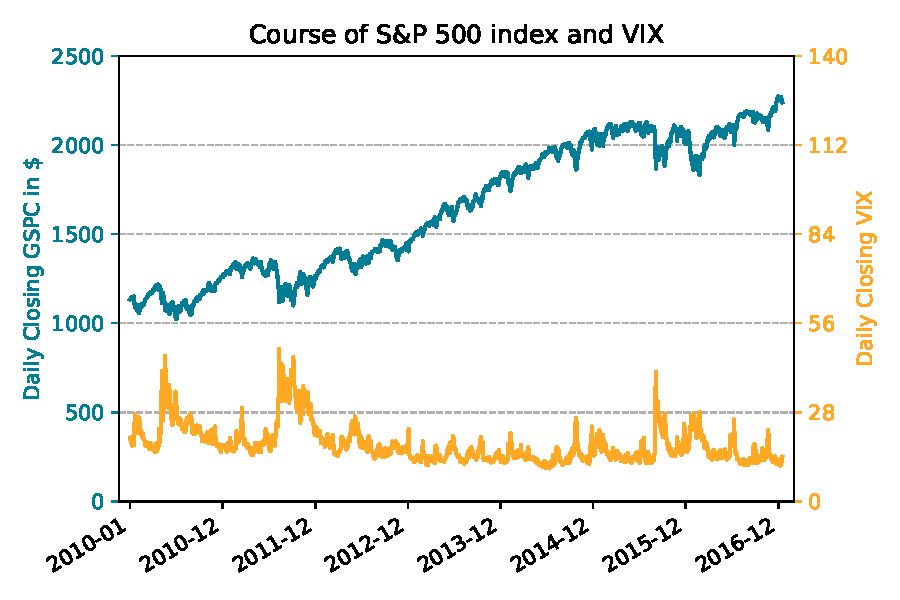
\includegraphics[width=0.8\textwidth]{figures/data/index-and-vix.pdf}
    \caption{Evolution of GSPC and VIX for the observed period. The scales are adjusted to visualize both time series close to each other in the same plot.}
    \label{fig:index_and_vix}
\end{figure}

The preselection ensures the complete stock prices of 467 companies for all 985 trading days from 2010-01-04 to 2013-11-29. % For evaluating prediction models all samples for the 189 trading days from 2013-03-01 on will be excluded during analysis and only used for final testing. The left over 794 trading days are used for the following analysis in Section~\ref{section:regression_analysis}.



% TODO: State: Only active trading days (holidays & weekends are excluded)


% Archived: Additionally it includes fundamental data extracted from Nasdaq Financials and SEC 10k annual fillings between 2012 and 2016. For each security essential information like ticker symbol, security name, address of headquarter, industry and sub industry are given.

\section{Statistical Analysis}
\label{section:statistical_analysis}
%%% Introduction:
This section is designed to calculate correlation (or cross-correlation) among stock prices. Therefore, the Pearson product-moment correlation coefficient, denoted as $r$, will be calculated for each pair of stock prices:

\newcommand{\return}[1]{r_#1^{(t)}}
\newcommand{\returnt}[2]{r_#1^{(#2)}}
\newcommand{\stock}[1]{s_#1^{(t)}}
\newcommand{\stockt}[2]{s_#1^{(#2)}}
\newcommand{\stockmean}[1]{\bar s_#1}

\begin{align}
    r = \frac{\sum _{t=1}^{n} (\stock{i} - \stockmean{i})(\stock{j} - \stockmean{j})}{\sqrt{\sum _{t=1}^{n} (\stock{i} - \stockmean{i})^2 }  \sqrt{\sum _{t=1}^{n} (\stock{j} - \stockmean{j})^2 }}
    \label{formula:pearson_r} \\ \eqname{Pearson's $r$}
\end{align}

where $\stock{i}$ and $\stock{j}$ are the preprocessed stock prices of two companies at trading day $t$ and $n$ is the sample size. $\stockmean{i}$ and $\stockmean{j}$ are the sample means.

Unfortunately, stock prices produce time series comprising characteristics like autocorrelation and heteroscedasticity which distort the results of statistical inference (Section~\ref{subsection:bg-statistics}). The analysis of economic variables, better known as econometrics, originated from the application of statistical methods on financial time series and deals with such problems to discover models and relationships among economic variables. To avoid spurious correlation \cite{Yule1926WhyTime-Series} and conclude with meaningful cross-correlation coefficients, this analysis conducts prewhitening methods from econometric and time series analysis on the collected stock prices.

For applying our analysis including hypothesis tests and regression models, we use the implementations by the python modules \emph{scikit-learn} \cite{Pedregosa2011Scikit-learnPython} and \emph{statsmodels}.

\subsection{Data Processing}
\label{subsection:data_processing}
% https://drive.google.com/file/d/18l7y9Oh9uEo6yANFsUDggIIaOPDYqsR1/view

In the following, the stock prices will be transformed to account for preconditions of correlation analysis since it requires independently and identically distributed (i.i.d.) samples \cite{Franke2010StatisticsMarkets}. The most important of those are not existing autocorrelation (also known as serial correlation) and homoscedasticity but also other constraints which will be examined after the data was fully processed. In the last preprocessing step, autoregressive models will be conducted to deal with remaining autoregressive patterns.

% MOVE TO AR: Before applying regression on time series, multiple characteristics need to be examined in advance since they can distort the results.
% In order to achieve a stationary variable, the original data is differenced vanishing the unit root.
% Autocorrelation can arise in various forms, e.g. unit root, trend-stationary or moving-average processes

\subsubsection{Stationarity}
\label{subsubsection:processing:stationarity}
Time series reveal roots which indicate the dependency on previous values. If the influence of such a root persists over time and prevents the series to return to a stationary mean, this root is called a unit root \cite{Engle1987Co-IntegrationTesting} and the series is designated non-stationary. Stock prices are assumed to contain a unit root \cite{LopezdePrado2018AdvancesLearning} which can be accounted for by differencing the time series. Depending on the data one uses, this can be done by taking the absolute or relative differences between each sample:

\begin{align}
    \Delta_i^{(t)} &= c_i^{(t)} - c_i^{(t-1)} \label{formula:abs_diff} \\ \eqname{Absolute Difference} \\
    \Delta_i^{(t)} &= \frac{c_i^{(t)}}{c_i^{(t-1)}} \label{formula:rel_diff} \\ \eqname{Relative Difference}
\end{align}

where $c_i^{(t)}$ is the unmodified closing stock price at trading day $t$.

To have comparable measures among stocks with different levels, the relative difference is used hereinafter. The selected dataset provides the open, close, high and low stock prices for each day so there are various ways to create returns, i.e. differences of the daily stock prices. \citet{Hong1998TradingClosures} provides empirical findings about recurring patterns in returns including that open-to-open returns are more volatile than close-to-close returns. \citet{Wang2009StatisticalReturn} provide evidence that intraday (open-to-close) and overnight (close-to-open) returns have significantly different properties concluding that one shall not mix them. \citet{Li2014NewsAnalysis} considers daily open-to-close prices arguing that it is less prone to seasonality and the more volatile non-trading gaps across weekends and holidays. 

The skewness and kurtosis of the current data investigated supports these findings. The distributions of open-to-open and close-to-close returns reveal a high kurtosis, conforming with related work that stock prices are leptokurtic \cite{Morgan1976StockHeteroscedasticity}. For the overnight returns extremely high kurtosis is observed upon the data used in this work. In contrast, the kurtosis of intraday returns is approximately three which equals the kurtosis of a normal distribution. For the skewness, we see a similar behaviour. The overnight returns revel a large negative skewness. While open-to-open and close-to-close returns substantiate a moderate negative skew (-0.1 in average) coinciding with related work, the intraday returns are distributed with a slightly positive skew (0.06 in average). Because of their more normal like distributions, intraday returns are used in the following which are calculated by the formula in Eqn.~\eqref{formula:return}. From a theoretical point of view, it is even more intelligible to select the returns across the period during high activity on the market. The returns are more likely to represent the impact of actual news and therefore reach faster a stable price level.

\begin{align}
    r^{(t)}_i &= \frac{c^{(t)}_i}{o^{(t)}_i}
    \label{formula:return} \\ \eqname{Intraday Return}
\end{align}

where $o_i^{(t)}$ and $c_i^{(t)}$ are the open and close prices for a stock at trading day $t$.


\subsubsection{Homoscedasticity}
\label{subsubsection:processing:homoscedasticity}
Another precondition for correlation is homogeneous volatility (variance in the context of time series), in the following denoted as homoscedasticity. The lack of this property is called heteroscedasticity. Unfortunately, stock prices are assumed to be heteroscedastic \cite{Morgan1976StockHeteroscedasticity}. In most cases, this can be addressed by modelling the time series with a generalized autoregressive conditional heteroscedasticity
(GARCH) model, using heteroscedasticity-consistent standard errors (e.g. Newey-West estimator) \cite{Millo2017RobustApproach} or applying robust regression methods (e.g. weighted least squares regression). If this not handled in any way, most test statistics tend to report biased results, e.g. the method of ordinary least squares (OLS) is not anymore the best linear unbiased estimator resulting in downwards biased coefficients \cite{Hallin2014Gauss-MarkovStatistics}. Usually, there can be various reasons for observing heteroscedasticity. For example. sensor data or data extracted from very noisy sources, such as text, may reveal measurement errors. In the context of stock prices, the heteroscedasticity is most likely caused by leaving out exogenous factors which will be treated in the following step of preprocessing.

% https://mpra.ub.uni-muenchen.de/54954/1/MPRA_paper_54954.pdf
% "Some statistical tests, for example the analysis of variance, assume that variances are equal across groups or samples. The Levene test can be used to verify that assumption."


One popular method for heuristic data stabilization is the Box-Cox transformation \cite{Box1964AnTransformations}. It is a simple power transformation which is applied on the calculated returns \eqref{formula:boxcox} to stabilize the data. It is assumed to mitigate heteroscedasticity, which will be examined in a later section. As suggested by \citet{Box1964AnTransformations}, the model's power parameter $\lambda$ is determined by maximizing the log-likelihood function.

\begin{align}
    r_i^{(t)(\lambda )} &={\begin{cases}{\dfrac {r_i^{(t)^\lambda}-1}{\lambda }}&{\text{if }}\lambda \neq 0,\\ \quad \ln r^{(t)}_i&{\text{if }}\lambda =0,\end{cases}}
    \label{formula:boxcox} \\ \eqname{Box-Cox Transformation}
\end{align}

where $r_i^{(t)(\lambda )}$ is the intraday return for a stock price at trading day $t$ after it was slightly adapted by a Box-Cox transformation with power parameter $\lambda$. In the following this transformed return is denoted as $r_i^{(t)}$ doe simplicity.


\subsubsection{Exogenous Variables}
\label{subsubsection:processing:exogenous}

As stated in the beginning of this study, financial markets are prone to manifold external influences which are usually not modelled during regressing stock prices. This type of mis-specification of leaving out exogenous variables in models is quite common, because they can not be observed directly or their inclusion increase the problem space in an excessively manner. Therefore, economic models usually focus on a few variables which are of high interest.

To account for those exogenous variables data normalization regarding the overall market behaviour is carried out. If the economy is doing well or experiences a period of uncertainty, this will be likely reflected in all stock prices. The selected stock prices are even part of the market index reflecting the overall market performance. Hence, omitting exogenous variable is another reason for spurious correlation \cite{Granger1969InvestigatingMethods}. A greater correlation between stock prices can be caused by a shared external factor which is the common market performance in this case. To have a better representation for the performance of a single stock, its returns needs to be normalized regarding the shared performance of the market. Further, the underlying movement of a stock price might even more be biased by the sentiment of the according industry section. Stocks from the same industry will therefore have a high cross-correlation without revealing a specific relationships, caused by the similar behaviour of investors in this section of the market.

In the following, the return value will be subtracted by the average return value of its industry sector:

\begin{align}
    \hat r^{(t)}_i &= r^{(t)}_i - \frac{1}{|B_{j}^{(t)}|} \sum \limits_{r^{(t)}_k \in B_{j}^{(t)}} r^{(t)}_k
    \label{formula:normalization} \\ \eqname{Industry Normalization}
\end{align}

where $B_{j}^{(t)}$ is a set of the transformed intraday returns at trading day $t$ for all companies in the same industry sector as the company for $r^{(t)}_i$. The resulting normalized intraday return $\hat r^{(t)}_i$ will be denoted in the following as $r^{(t)}_i$.


Normalizing by the S\&P~500 market index instead of the separate industry means will be examined by the distribution of resulting cross-correlations in Section~\ref{subsection:cross_correlation}.
\subsubsection{Autoregression}
\label{subsubsection:processing:ar_modelling}

Even though, differencing and normalization successfully remove some autocorrelations, autoregressive patterns can remain which can be accounted for by autoregressive models. In contrast to their most popular application (e.g. \citet{Ruiz2012CorrelatingActivity}), autoregressive models are not used for forecasting purposes. They are simple linear models with unrealistic constraints and thereby far exceeded by machine learning models \cite{Hsu2016BridgingEconomists}. Nevertheless, they are able to model the linear autoregression of time series which shall be filtered out before cross-correlating time series. If a temporal variable reveals autoregression, a value within this time series can be described by a function of its past values plus an error term $\epsilon$ which is also known as residual. If such autoregression is present for two correlated time series, the calculated correlation coefficient is found to be invalid. Instead, a suitable autoregressive model shall be applied and correlation analysis conducted on the residuals because they are assumed to be free from linear autoregression.

% "Regression models for prediction are often useful even when the assumptions are moderately violated, although they may not perform optimally. However, in many applications, especially with small effects or questions of causality based on observational data, regression methods can give misleading results.[2][3]" (https://en.wikipedia.org/wiki/Regression_analysis)

% History of Time Series Analysis, Types of interventions (omitted vars.), etc. --> https://autobox.com/cms/index.php/afs-university/intro-to-forecasting/doc_download/1-the-autobox-advantage

\paragraph{ARMA}
To remove autoregressive patterns in the mean of the process, an autoregressive-moving-average (ARMA) model is applied \cite{Dionisio2004MutualSeries}. It assumes a temporal observation to be linear combination of the $p$ lagged values and the $q$ lagged error terms from the same stationary and univariate time series \eqref{formula:ar_model}. The remaining value, in the following residual, which cannot be modelled by these terms is called the error term and is assumed to be i.i.d. It should not reveal any significant autocorrelation if an appropriate ARMA model was selected and therefore is valuable for further correlation analysis avoiding spurious correlation \cite{Yule1926WhyTime-Series}. A common approach for determining the hyper parameters, known as Box-Jenkins method \cite{Box1970TimeControl}, uses the autocorrelation function (ACF) and partial autocorrelation function (PACF) \cite{Franke2010StatisticsMarkets}. The ACF describes the correlation of an observation with lag values. The PACF has the same focus but uses a statistically adjusted correlation that is not accounted for by intermediate lags. For the model identification, the number of significant correlation lags from the PACF determines $p$ while the number from the ACF determines $q$. The resulting model is denoted as ARMA(p, q).

% https://machinelearningmastery.com/gentle-introduction-autocorrelation-partial-autocorrelation/
% https://ncss-wpengine.netdna-ssl.com/wp-content/themes/ncss/pdf/Procedures/NCSS/The_Box-Jenkins_Method.pdf
% https://www.academia.edu/2099523/Time_series_analysis_forecasting_and_control
% https://machinelearningmastery.com/gentle-introduction-box-jenkins-method-time-series-forecasting/

\begin{align}
    \returnt{i}{t} &= \sum \limits_{j=1}^{p} a_j \returnt{i}{t-j} + \sum \limits_{j=1}^{q} b_j \epsilon_{t-i} + \epsilon_t  \label{formula:ar_model} \\ \eqname{ARMA Model}
\end{align}

The intraday return at $t$ is regressed by $p$ lagged values $\returnt{i}{t-p}, ..., \returnt{i}{t-1}$ and $q$ lagged error terms $\epsilon_{t-q}, ..., \epsilon_{t-1}$. In order to do so, the model coefficients $a_1, ..., a_p$ and $b_1, ..., b_q$ are fitted with OLS. $\epsilon$ denotes the residual representing the part of $\returnt{i}{t}$ which can not be described by autoregression and therefore is considered to be free of autocorrelation. In the following, the model residual is denoted with $\returnt{i}{t}$. It also involves those stock returns for which no autoregressive modelling was required.

\begin{figure}[!ht]
    \centering
    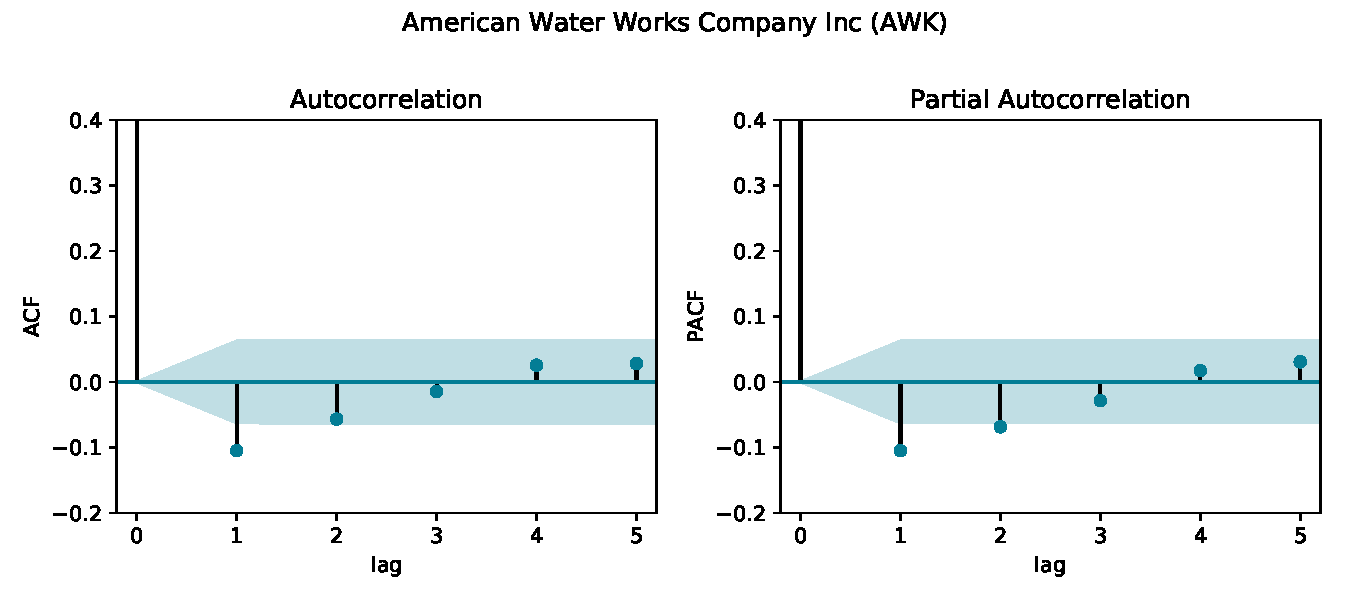
\includegraphics[width=\textwidth]{figures/regression/acf-awk-normed.pdf}
    \caption{ACF and PACF plots for the preprocessed stock returns for company \emph{American Water Works Company Inc}. The x-axis shows the lag and the y-axis shows the correlation coefficient (Pearson's $r$). The colored area around zero represents the 0.95 confidence interval of no significant correlation. All values out of this range can be assumed to be correlated. The autocorrelation of a zero lag will always be one, so the plots are adjusted to not fully show this dispensable data point but put more focus on the following lags.}
    \label{fig:acf_pacf_awk_normed}
\end{figure}

For 385 stocks there was no autocorrelation observable so the ARMA model was not applied on this data. To show an example how lags are determined and how the modelling reduces autocorrelation, the ACF and PACF are plotted in Figure~\ref{fig:acf_pacf_awk_normed} for an example company. The ACF shows significance for one lag while the PACF even shows significance for two lags, so an ARMA(2, 1) model will be applied.

\begin{figure}[!ht]
    \centering
    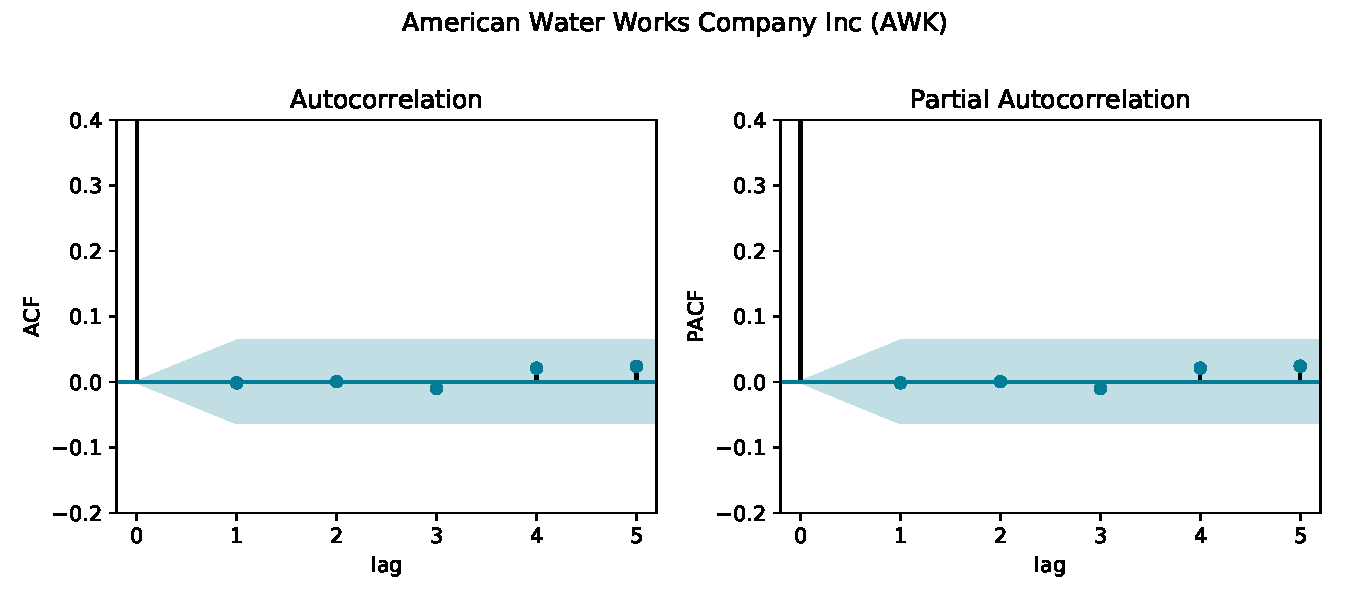
\includegraphics[width=\textwidth]{figures/regression/acf-awk-resid.pdf}
    \caption{ACF and PACF plots for the preprocessed stock returns for company \emph{American Water Works Company Inc} after taking the residuals of an ARMA(2, 1) process.}
    \label{fig:acf_pacf_awk_resid}
\end{figure}

Figure~\ref{fig:acf_pacf_awk_resid} shows the same plots for ACF and PACF after the autoregressive process was filtered out. There is no significant autocorrelation left, so the modelling was successful. To inspect the outcome of this modelling, later evaluation will investigate the autocorrelation of residuals extracted from those ARMA models. If no model was applied because it was not appropriate, the time series is still treated as the residuals of a mean process justifying the usage of the following model for volatility.

\paragraph{GARCH} In the last step of preprocessing, the autoregressive patterns in volatility are modelled which needs to be done additionally to the previous mean modelling by ARMA models. The generalized autoregressive conditional heteroscedasticity (GARCH) model \cite{Bollerslev1986GeneralizedHeteroskedasticity} is a way to treat the unstable volatility in stock prices which are already assumed to be not mean autocorrelated, stationary and without structural breaks. It is applied on the residuals of a mean process which resulted from the previous ARMA(p, q) modelling. The GARCH(u, v) model approximates the residual's volatility $\sigma^2(t)$ (standard deviation over time) by a linear combination of $u$ previous volatility values and $v$ previous residuals, as shown in formula~\eqref{formula:garch_model}: % The parameter $\omega$ denotes the constant volatility over the whole process.

\begin{align}
    {\sigma_i^{(t)}}^2 &= \sum \limits_{j=1}^{v} c_j {\returnt{i}{t-j}}^2 + \sum \limits_{j=1}^{u} d_j {\sigma_i^{(t-j)}}^2 + \omega \label{formula:garch_model} \\ \eqname{GARCH Model}
\end{align}

where $\omega$ is the constant volatility over the whole time series, $\returnt{i}{t-v}, ..., \returnt{i}{t-1}$ are the considered residuals of the previous ARMA model and ${\sigma_i^{(t)}}^2$ is the volatility of $\returnt{i}{t}$ at trading day $t$. The model coefficients for incorporating lagged residuals and volatility are $c_1, ..., c_v$ and $d_1, ..., d_u$.

For estimation of the hyper parameters $u$ and $v$ of a GARCH(u, v) model, a similar method as for ARMA(p, q) is conducted on the squared residuals which are supposed to be zero-mean. Because the actual volatility cannot be directly observed, the squared residuals are commonly used as a proxy. Depending on the number of lags of significant (partial) autocorrelation, $u$ and $v$ are chosen. % There are other approaches for determining parameters of a GARCH model like using an Information Criterion which measures the suitability of model.

To conclude with homoscedastic data for the following correlation analysis, the standardized residuals are calculated from this model by dividing the previous ARMA residuals by the conditional volatility calculated with the GARCH model, as shown in Formula~\eqref{formula:std_resid}. The stocks, for which no GARCH model was applied, are divided by their overall standard deviation to keep the time series in the same scale. It is important to mention that this will not affect the results since the same scalar is used for all values of the time series.

\begin{align}
    \stock{i} &= \frac{\return{i}}{\sigma_i^{(t)}}
    \label{formula:std_resid} \\ \eqname{Standardized Residuals}
\end{align}

where $\stock{i}$ is the final variable which will be used in the following for time series analysis. It incorporates both model residuals and rectified intraday returns depending on whether a model was applied or not.

\begin{figure}[!ht]
    \centering
    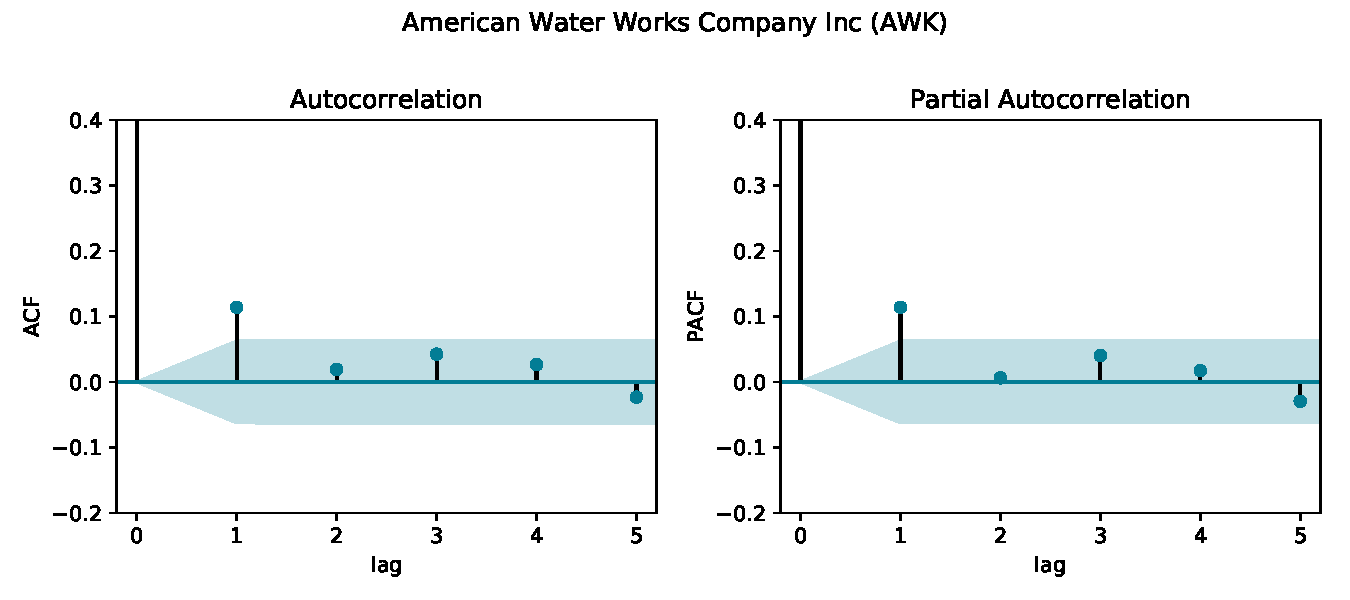
\includegraphics[width=\textwidth]{figures/regression/acf-awk-resid-sqr.pdf}
    \caption{ACF and PACF plot for the squared residuals after applying a ARMA(2, 1) model on the preprocessed stock returns for company \emph{American Water Works Company Inc}.}
    \label{fig:acf_pacf_awk_resid_sqr}
\end{figure}

Figure~\ref{fig:acf_pacf_awk_resid_sqr} visualizes the ACF and PACF for the approximated volatility of an example company by using its squared preprocessed stock returns. The ACF and PACF both reveal significance for the first lag only. This leads to the suggestion of applying a GARCH(1, 1) model.

\begin{figure}[!ht]
    \centering
    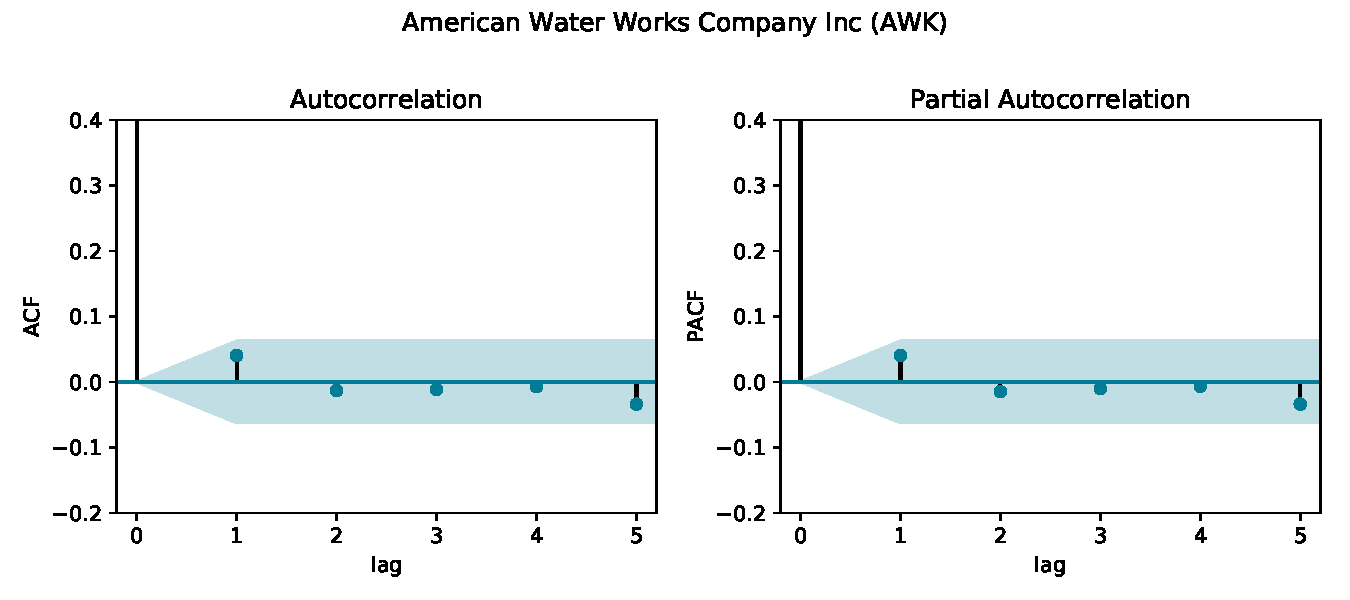
\includegraphics[width=\textwidth]{figures/regression/acf-awk-std-resid-sqr.pdf}
    \caption{ACF plot for the squared residuals after applying a ARMA(2, 1) and a GARCH(1, 1) model on the preprocessed stock returns for company \emph{American Water Works Company Inc}.}
    \label{fig:acf_pacf_awk_std_resid_sqr}
\end{figure}


To evaluate the success of the approach, the ACF and PACF of the standardized residuals are shown in Figure~\ref{fig:acf_pacf_awk_std_resid_sqr}. Clearly, the autocorrelations of the considered lag and even some following lags diminished to a insignificant level close to zero. Under the same procedure, the need of modeling volatility and selection of suitable hyper parameters is examined on all 467 stocks. For 306 from these a GARCH model is applied, usually with $u=1$ and $v=1$.



% The autoregressive–moving-average (ARMA) modelling requires stationarity for calculating its slope coefficients. They are usually calculated using Ordinary Least Squares (OLS) \cite{GrangerNewbold}.


% FORECAST WITH FEASIBLE MODELS: Based on the previously found properties select model (LR, ARIMA, EGARCH, GARCH, etc.). Evaluate models with MAPE (include Diebold and Mariano (DM) test?) and information criterion (AIC, BIC, HCQ). (parametric: ARIMA vs. non-parametric: Link relatives, difference)
%   A) ARIMA parameters can be estimated by finding last significant lag in ACF & PACF. Afterwards evaluate by inspecting "Residual vs fitted" chart and ACF of the models residuals https://newonlinecourses.science.psu.edu/stat510/node/47/
%   B) For predictions: persistence model as baseline

% \subsubsection{Exogeneous Variables}
% Taking GSPC & industry into account as exogeneous variables enables us to reflect other external influences which have an impace on the whole market.


\subsection{Time Series Evaluation}
\label{subsection:time_series_evaluation}
After the stock prices were differenced, stabilized, normalized and autoregressively modeled, characteristics of the resulting time series will be examined. While there are easy to apply methods for establishing stationarity and removing trends, some characteristics like structural breaks are most likely hard to remove. Therefore, in some cases not all preconditions are ensured. But the data is not further transformed to enforce less outliers, removed periodicity or ensure ergodicity. By applying yet another transformation in order to achieve those conditions, the data might be polluted in a too drastic way. However, one should be aware of the level of violations for assumptions which are required in correlation analysis.

\begin{figure}
    \centering
    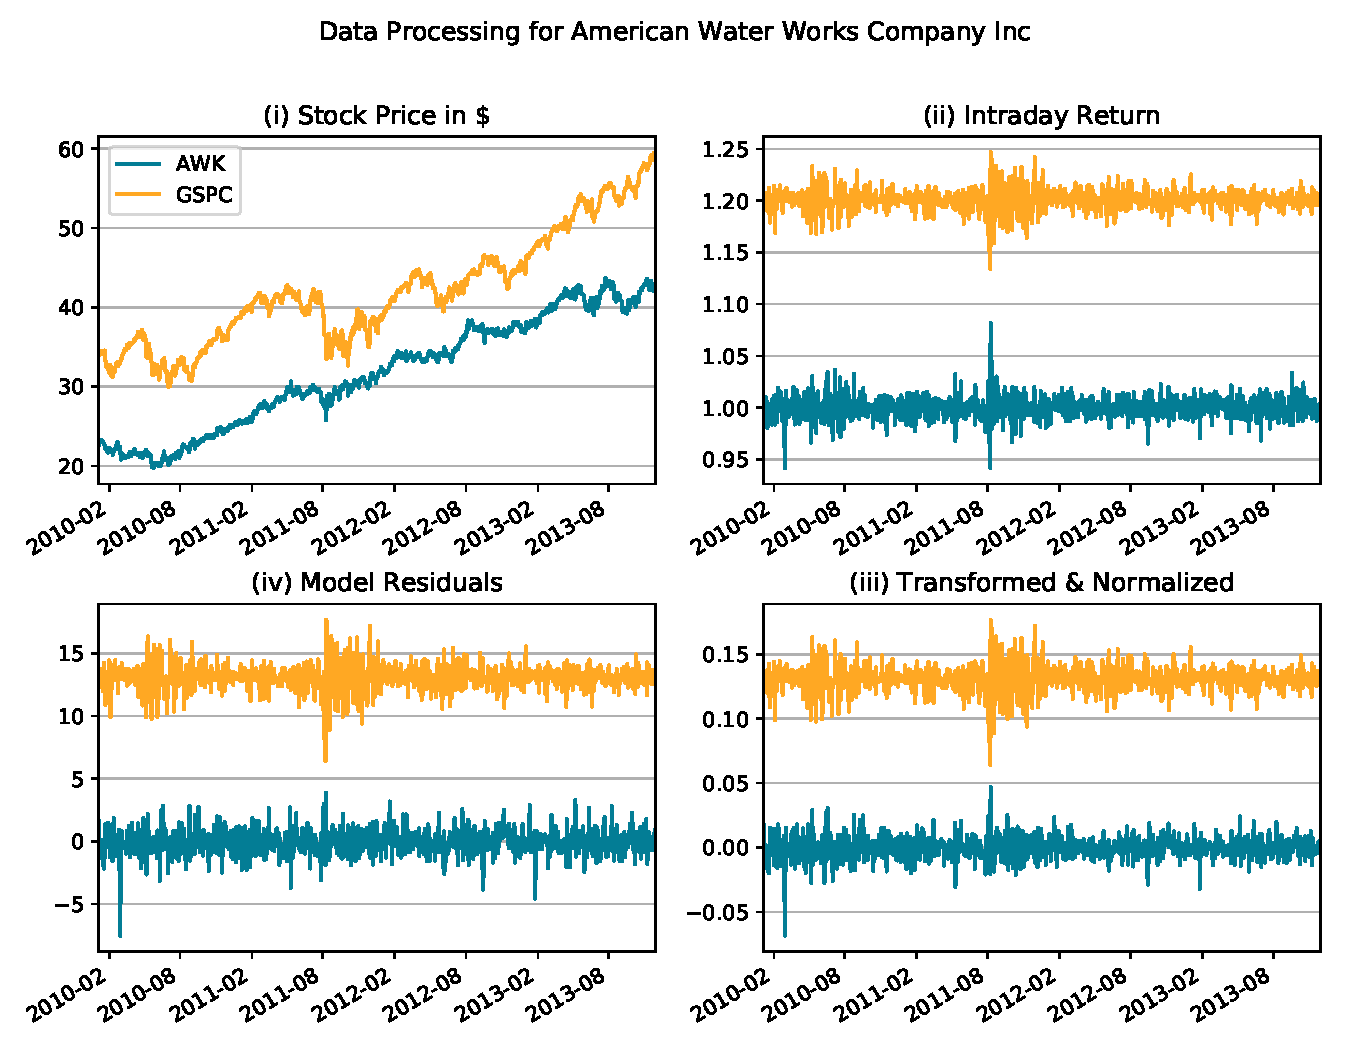
\includegraphics[width=0.9\textwidth]{figures/regression/data-processing-awk.pdf}
    \captionsetup{singlelinecheck=off}
    \caption[foo bar]{Values from intermediate preprocessing steps for the company \emph{American Water Works Company Inc} are shown in blue and compared with the price or intraday return of the S\&P~500 market index in orange. In all cases, the index was scaled and shifted in order to show both time series next to each other. The preprocessing steps are arranged clockwise, starting from the top left corner: \begin{enumerate*}[label=(\roman*)]
        \item unmodified stock prices,
        \item intraday returns,
        \item stabilized and industry-wise normalized returns and
        \item standardized residuals of ARMA(2, 1) and GARCH(1, 1) models on returns.
    \end{enumerate*}}
    \label{fig:data-processing-steps}
\end{figure}

Figure~\ref{fig:data-processing-steps} visualizes the impact of preprocessing on a stock price and takes the S\&P~500 market index into account. In the first plot both time series move strongly similar. After taking the intraday returns, stationarity appears to be ensured but both time series still tend to reveal similarity, e.g. by simultaneous bursts or change in volatility. Subsequently, the return values are stabilized with Box-Cox transformation and normalized by the regarding industry mean. Even though some parts still indicate an existing relationship, the time series is located more stable around zero and reveals less outlier. In the last step, the volatility is adjusted by ARMA and GARCH modelling, resulting in a time series which appears to be very similar to a white noise. Since a white noise process is considered to fulfill almost all constraints in order to be i.i.d., the data seems to be promising for further analysis.


\subsubsection{Stationarity}
\label{subsubsection:stationarity}

The stationarity is one of the most important properties one need to examine before conducting further time series analysis. If it is not present, experiments like correlations or ARMA models lead to falsely results. The stationarity is evaluated by applying hypothesis tests for the presence of unit roots on the examined time series. It is recommended to apply multiple hypothesis tests to provide assurance of a correct outcome, so we will execute the following ones:
\begin{enumerate*}[label=(\roman*)]
    \item Augmented Dickey-Fuller (ADF) \cite{Dickey1976IntroductionSeries}
    \item Phillips-Perron (PP) \cite{Phillips1988TestingRegression}
    \item Kwiatkowski–Phillips–Schmidt–Shin (KPSS) \cite{Kwiatkowski1992TestingRoot}
\end{enumerate*}

The first two test the null hypothesis, that a unit root is present. In contrast, the latter one tests the null hypothesis of stationary data. As common practice (e.g. \cite{Bishara2012TestingApproaches}), the significance level $\alpha=0.05$ is defined for the $p$-value in order to sufficiently reject the null hypothesis.

All three tests are executed on all 467 stock prices at each step of their preprocessing stage. Except for 14 cases, all three tests attest the presence of a unit root in the original stock prices. After taking the intraday returns, there is no stock, for which all three tests simultaneously give evidence for a unit root. Only the KPSS test significantly rejects the absence of unit roots for 15 cases. The following preprocessing steps did not change this number by large, so the final time series can be expected to be stationary.

% "Any series that has a trend will tend to be correlated to any other series that has a trend. For this reason, it is preferable to remove trends and seasonal effects before comparing multiple series. This is usually achieved by working with the residuals of a fitted time series model, such as the regression models of Chapter 3" (Introductory Time Series With R, Cowpertwait and Metcalfe )

% "The model should only be applied to a prewhitened residual series {e_t} that is uncorrelated and contains no trends or seasonal changes, such as might be obtained after fitting a satisfactory SARIMA model." (Cowpertwait and Metcalfe, Page 148, Introductory Time Series with R, 2009)

% RESOLVE unit root: If it cannot be rejected one may run the same test after applying a difference operator like AR(1), AR(2) or Link relatives.
% Diagnostic checking on residuals for:
%   A) Normality 
%   B) Autocorrelation 
%   C) Het.Sce. 
%   D) Test for structural breaks?
%   E) Other properties like periodicity, seasonality and outliers

% Even though there are a lot of factors influencing the stock markets behaviour one needs to cut it down to a few more important variables. Omitting influencing exogeneous factors might lead to spurious correlations / endogeneity but we need to reduce the dimensions of freedom avoiding curse of dimensionality (what is endogeneity: https://www.statisticshowto.datasciencecentral.com/endogenous-variable/) -> Check for endogeneity (error term correlates with independent variable within the model). This would mean that the model is biased and regression analysis using OLS is erroneous. Possible reasons for endogeneity: ommited variables; Measurement error in variable (noise is considered to be part of variable) -> OLS estimation will be biased downwards; Simultaneity (fixed by Instrumental Variables Regression)

% UNIT ROOT: Is it unit root? (explained in background) Apply ADF, PP and/or KPSS as \cite{Vlastakis2012}. Differentiate between trend-stationary, difference-stationary and just non-stationary. If and only if the null hypothesis of unit root can be rejected, one can apply autoregression; "A finding of a unit root implies that stock returns cannot be predicted." \cite{Narayan2005}. Unit root processes are tíme-series which do not fully recover from shocks. The term originates from a coefficient equal to one for the last value when the next value is calculated, hiding/covering the underlying trend ones is looking for.


\subsubsection{Data Distribution}
\label{subsubsection:normal_dist}

% Many financial variables are non-normally distributed (Mandelbrot and Benuit 1963)

Another precondition of cross-correlation are normal distributed samples \cite{Bishara2012TestingApproaches}. For evaluating if the data distribution is similar to a normal distribution, again hypothesis tests are a good way to acquire evidence in favour of or against normality being present. For example, \citet{Vlastakis2012InformationVolatility} use the Jarque-Bera test \cite{Jarque1980EfficientResiduals} to inspect the null hypothesis that a normal distribution is present. Conducted on the 30 stocks from Dow Jones Industrial Average, they reject the presence of a normal distribution with 99~\% confidence. As stated in the previous section, it is a common practice to use multiple tests for double-checking the results. For this task, the following are applied which all rely on the same null hypothesis of normality being present:
\begin{enumerate*}[label=(\roman*)]
    \item Jarque-Bera (JB) \cite{Jarque1980EfficientResiduals}
    \item Shapiro-Wilk (SW) \cite{Shapiro1965AnSamples}
    \item D’Agostino’s K\^2 (DK2) \cite{DAgostino1973Testsb}
    \item Anderson-Darling (AD) \cite{Stephens1974EDFComparisons}
\end{enumerate*}

As might be expected from the initial analysis of kurtosis and skewness in Section~\ref{subsubsection:processing:stationarity}, only 16 out of 467 preprocessed stock prices reveal evidence for a normal distribution by at least one test statistic.


To inspect the possibility of another distribution, the Kolmogorow-Smirnow (KS) \cite{Massey1951TheFit} test is applied. It assesses the equality of two distributions by calculating the distance of their cumulative distribution function. The distributions of each preprocessed stock prices is compared to a set of common probability distributions. The most frequently distribution (using a rejection rate of $\alpha=0.05~\%$) was Student's $t$ with 7 dimensions of freedom in average, followed by logistic, laplace and normal distribution. Based on the suggested distributions, the data appears to have heavier tails as a normal distribution. % Still, the normal distribution appears to be a reasonable assumption for 304 out of 467 preprocessed stock return series and the close average kurtosis and skewness provide evidence for the suitability. Except for the examination of outliers, the data will therefore be treated as a normal distribution.

These findings do not lead to the conclusion that calculating the correlation on such non-normal data returns erroneous conclusion. The Pearson correlation coefficient, which will be introduced later, is fairly robust for different data distributions, although it does assume normality. Only if the distribution differs strongly from normality, e.g. by extreme values for skew or kurtosis, it should be treated with caution \cite{Bishara2012TestingApproaches}.

% https://sci-hub.se/10.2466/pms.1976.43.3f.1319


\subsubsection{Homoscedasticity}
\label{subsubsection:homoscedasticity}

Economic variables like stock prices are known to potentially exhibit heteroscedasticity \cite{Salisu2016UnitSeries}. To examine linear versions of heteroscedasticity, the Breusch-Pagan test (BP) \cite{Breusch1979AVariation} can be used. If this test fails to reject the null hypothesis of homoscedasticity and therefore indicates the presence of homoscedasticity, the White test \cite{White1980AHeteroskedasticity} can be applied to test for nonlinear forms. It checks the null hypothesis on a greater set of terms which needs more calculation and might reveal less significant results than BP. Because of the large number of degrees of freedom, the White test can over-react. Concluding, both tests are applied in the following. % https://www3.nd.edu/~rwilliam/stats2/l25.pdf

While at least one test indicated heteroscedasticity for 422 stocks based on their intraday return values, 307 remained with significant results after transformation and normalization. The enhanced stability in form of volatility, gives subsequent justification for the previous prewhitening steps. In more than a half of these cases the White test revealed sufficient evidence while the BP did not. This leads to the conclusion that in many cases the data contains nonlinear heteroscedasticity, which BP is not able to detect.

After applying the GARCH model, 28 stocks remain which do not satisfy both tests for homoscedasticity. Besides those 28 stocks, 94 stocks have at least one test showing evidence for rejecting the null hypothesis. Most of these show evidence for the White test. Since this leads to the conclusion that there is still nonlinear heteroscedasticity present, the GARCH model might be not the best model and a more sophisticated approach like a nonlinear GARCH might be more suitable in future work. However, a large proportion of heteroscedasticity was removed compared to the original stock returns.

% (White Test with stats.diagnostic.het_white [from https://machinelearningmastery.com/develop-arch-and-garch-models-for-time-series-forecasting-in-python/)], BP test including the squared value, Engle's ARCH test (null=homo), Levene's Test -> https://sci-hub.se/10.2307/2328672) 

% (https://www.researchgate.net/post/How_to_remove_serial_correlation_and_heteroskedasticity) (https://mpra.ub.uni-muenchen.de/54954/1/MPRA_paper_54954.pdf) (https://sci-hub.se/10.1080/00036840802600087)

\subsubsection{Structural Breaks}
\label{subsubsection:structural_breaks}

% Additionally, the following analysis inspects the time series on structural breaks like shifts or bursts, and heteroscedasticity (heterogeneous volatility) \cite{xxxSalisu2016}.

Regression models, which are broadly used for hypothesis testing and other purposes, are established by estimating the coefficient of regressors fitting the dependent variable. A big issue of such coefficients are their stability. If the regressed variables contain structural changes like a level shift in mean or volatility, the estimated coefficients are most likely to be not suitable. If a specific point of time should be examined regarding a structural break, tests can be used which compare the regression coefficients which are calculated separately on each half of the dataset. If the coefficients are sufficiently different from each other, the time series can be assumed to have a structural break at the chosen time stamp.

However, examining the existence of structural breaks in an unsupervised manner, i.e. at an unknown point of time, appears to be a more difficult topic. Even, the application of machine learning for unsupervised anomaly detection is an ongoing topic, which is not completely reliable. All the more, the automated check using a statistical approach should be viewed skeptical. Therefore, only evidence for the presence of an unknown number of structural breaks is collected. The work will not further deal with it, accepting their presence for a few cases. The CUSUM-test \cite{Brown1975TechniquesTime} can be used for these cases, testing the null hypothesis of stable coefficients of a linear regression model.

Only two out of all original stock prices are assumed to contain at least one structural break following the CUSUM-test. The number increases only slightly after differencing and normalization concluding with 22 stocks revealing unstable coefficients. Even though, we are trying to remove the mean movement across one industry, not all prices might contain this common behaviour for the entire period. For some stock prices, the normalization step appears to introduce a new movement sectionally which leads to the significant rejection of stable coefficients over the entire times series.

\subsubsection{Autocorrelation}
\label{subsubsection:autocorrelation}

To test the autocorrelation across the whole dataset, two hypothesis tests were applied. The Durbin-Watson statistic \cite{Durbin1971TestingRegression.III} returns a number between 0 and 4 with suggesting no autocorrelation for the first lag if the statistic falls between 1.5 and 2.5. The Ljung-Box Q Test \cite{Dionisio2004MutualSeries} was also applied on the first lag only and tests the null hypothesis of no autocorrelation. Before applying autoregressive models, the preprocessing already reduced the number of first-lag autocorrelated stock returns from 467 down to 82 which was also observed previously by looking at the significant lags of ACF and PACF in Section~\ref{subsubsection:processing:ar_modelling}. For these remaining cases, the modelling was applied and successfully cleared the autocorrelation completely for all time series.

\subsubsection{Further Properties}

Variables and their regarding distributions are hard to describe without visualizing the data. descriptive properties like skewness, kurtosis and heteroscedasticity are provided, but they can not fully reflect the data itself. Even though stationarity is validated, latent periodic patterns can still remain.

\paragraph{Seasonality} 
Following the decomposition model, some autoregressive patterns can be describes by seasonality (recurring at fixed time intervals) or cyclicality (recurring patterns without fixed time frames). Since the data preprocessing does not account for these properties, it needs to be conducted if there is evidence for such periodic patterns. Especially, daily prices are prone to seasonality in form of weekly, monthly or seasonal patterns. Since two stock prices might follow the same pattern, there is always a chance of falsely correlating stock prices. Related work suggests using a differencing window over a year, so only two days from the same time of a year are always compared. Despite of a sliding window, this would decrease the number of resulting data points by about 250 samples (number of trading days in one year) which is critical for the size of the dataset used in this work.

% Seasonality can be fixed by increasing the differencing window (e.g. diff over a year to fix months). Microscopic patterns (e.g. on a weekly basis) are hard to detect.  Finding sporadic occurring patterns, seasonality or periodicity in noisy data like stock prices is a difficult topic, missing a panacea for the correct method. Even though, those characteristics should be considered in regression analysis, you never can be sure to have them removed and work on clean un-autocorrelated data. e.g. for expected seasonality: December Effect (https://www.timothysykes.com/blog/seasonal-stocks/)

\begin{figure}[!ht]
    \centering
    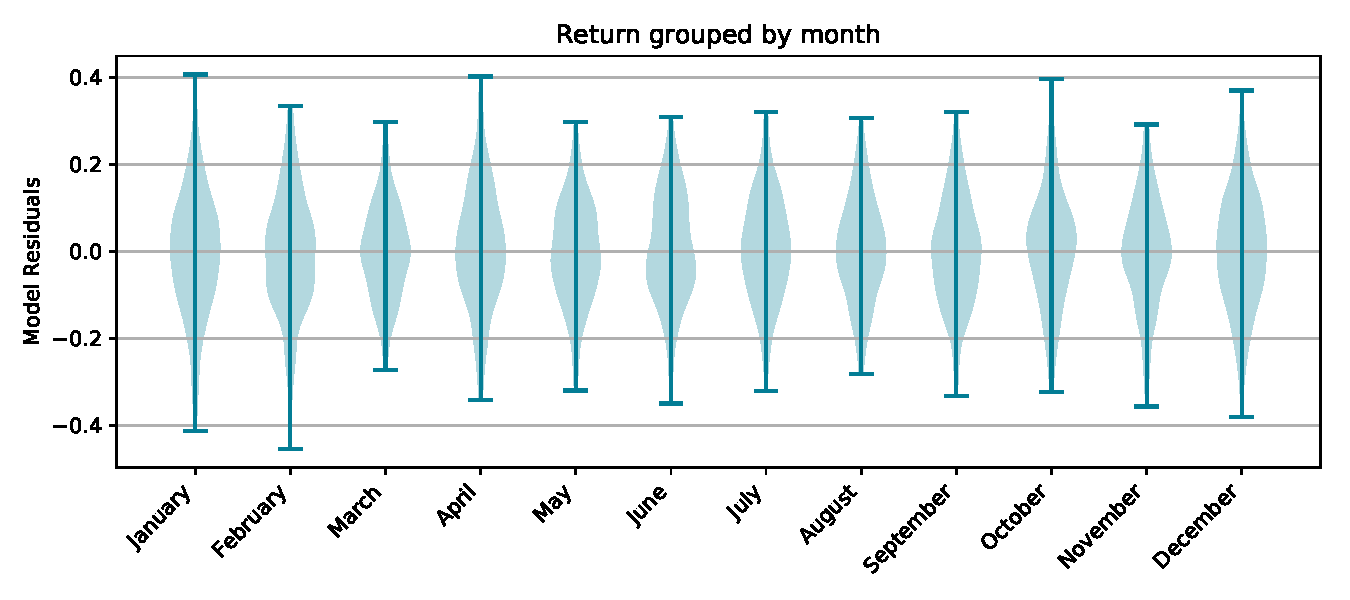
\includegraphics[width=\textwidth]{figures/regression/returns-per-month.pdf}
    \caption{Violin plot of preprocessed return values, denoted as model residuals, after taking the mean for each month and stock. The filled area visualizes the approximated data distribution along the vertical line}
    \label{fig:boxplot_seasons}
\end{figure}

Figure~\ref{fig:boxplot_seasons} shows the averaged model residuals for each month and stock. For every month the mean is not significantly different from zero but the standard deviation partially varies across the year. The lowest standard deviation is observed for the 467 values in March which equals 0.0998. The highest standard deviation 0.1266 is observed for January indicating a slightly increased uncertainty after the Christmas business. However, these result shows that there is no observable seasonality measured upon the mean monthly values. The same analysis was conducted for separate industries, too. While there is a significant seasonality visible on the original returns, they disappear after normalizing by the industry-wide mean, leading to similar zero-mean distribution as in Figure~\ref{fig:boxplot_seasons}.


\paragraph{Outliers}
Outliers are usually described as unexpected data points with an abnormal distance from the center of the data. The removal of such outliers is common but questionable practice since it can affect data properties. Unfortunately, there it is not easy to determine outliers in a non-parametric fashion for an arbitrary data distribution. A Student's $t$-distribution is most likely to fit the acquired data as pointed out before. Similar to the interquartile method for a normal distribution, an observation is seen as an outlier if it exceeds a chosen confidence interval. Suitable values for the distribution parameters (dimension of freedom, location and scale) are determined for each stock separately. Based on these parameters, the 99.5~\% confidence interval is calculated. Per definition, only 0.5~\%, i.e. five out of 984 observations, ought to be outside of this interval. On the preprocessed data, 199 stocks contain more than five outliers, but no more than seven.

\begin{figure}[!ht]
    \centering
    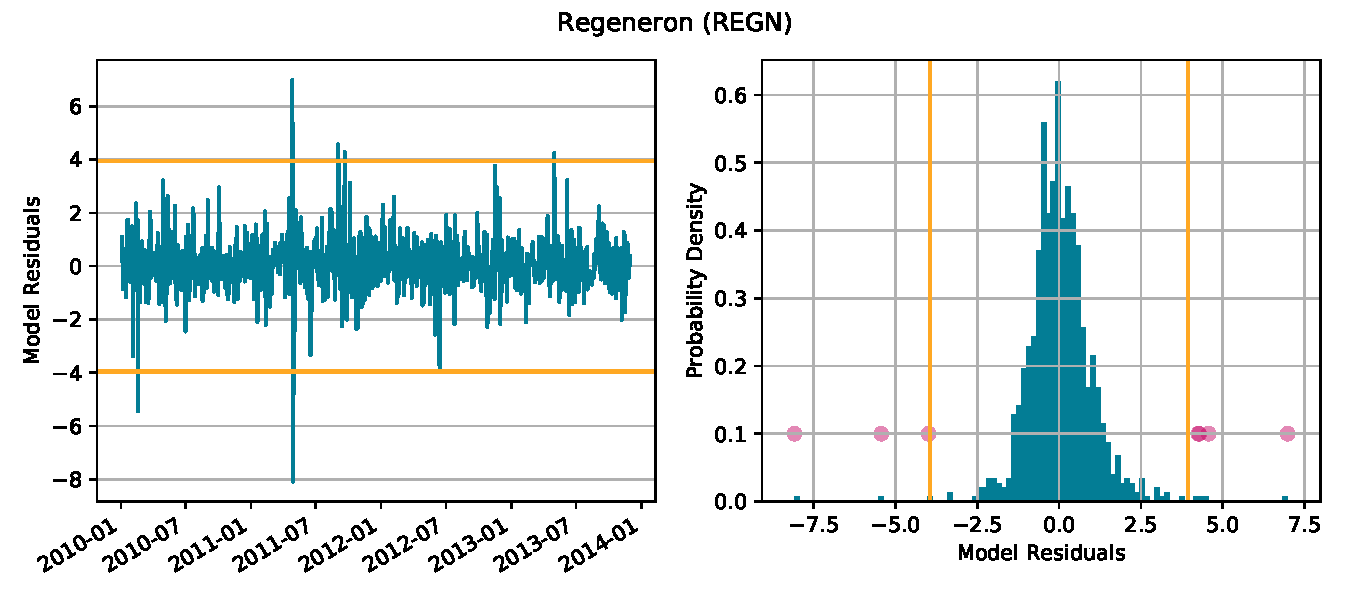
\includegraphics[width=\textwidth]{figures/regression/data-outliers-REGN.pdf}
    \caption{Preprocessed stock return and density histogram of those values for company \emph{Regeneron}. The orange line denotes the 99.5~\% confidence interval for a Student's $t$ distribution with four dimensions of freedom. On seven days an extreme value was observed which is denoted by a purple circle in the histogram on the right. The greatest two outliers can be observed for the 27th of April, 2011.}
    \label{fig:data_outliers}
\end{figure}

One stock with seven outliers is shown in Figure~\ref{fig:data_outliers}. At the 27th of April in 2011, the stock underwent a fast increase and decrease in value. This anomalous behaviour was caused by a successful study regarding a new drug for treatment of advanced colorectal cancer. The article \emph{\enquote{Regeneron, Sanofi Therapy Extends Lives of Colorectal Cancer Patients}} by Bloomberg, published in the evening of the 26th of April, reported these results.
 
Because removal or scaling down of unexpected extreme values, transforms the data in an unreasonable fashion and because it is not feasible to determine which data point should be considered actually unexpected, the outliers will not be treated different from the other data points. However, it is still worth mentioning that the number of outliers is not far above the expected value and therefore considered to not raise a sufficient influence on the data analysis.

% On the basis of a normal distribution, an observation would be to assumed to be an outlier if it falls below $Q1-1.5\times IQR$ or above $Q3+1.5\times IQR$, where $Q1$ and $Q3$ refer to the first and third quartile and $IQR$ to the interquartile range of the data.

% On the residuals, again the full analysis of characteristics was executed. In terms of stationarity, data distribution, heteroscedasticity, structural breaks and outliers no substantial change was observed.

\subsection{Time Series Correlation}
\label{subsection:cross_correlation}
Until this point, this section mainly focused on establishing statistical preconditions before it is possible to acquire cross-correlation. If the previous steps would be left out, the correlation would be much more likely to report erroneous results, e.g. spurious correlation. For calculating a bivariate correlation, Pearson's $r$ \eqref{formula:pearson_r}, will be used in the following.

% https://drive.google.com/file/d/1EKf_rly5OQ-oTts61HDeddYCwuBZLd1n/view

In order to make the danger of spurious correlation more tangible, Figure~\ref{fig:spurious_regression} shows an example for two stock prices which are not preprocessed. While the correlation on the plain stock prices appears very high with $r=0.96$, it is rather not existing at all after the preprocessing steps of differencing, transformation, normalization and modelling. This indicates that the first observed $r$ is high due to the autocorrelation of the both time series and their shared exogenous variable, i.e. the overall market performance.

\begin{figure}[!ht]
    \centering
    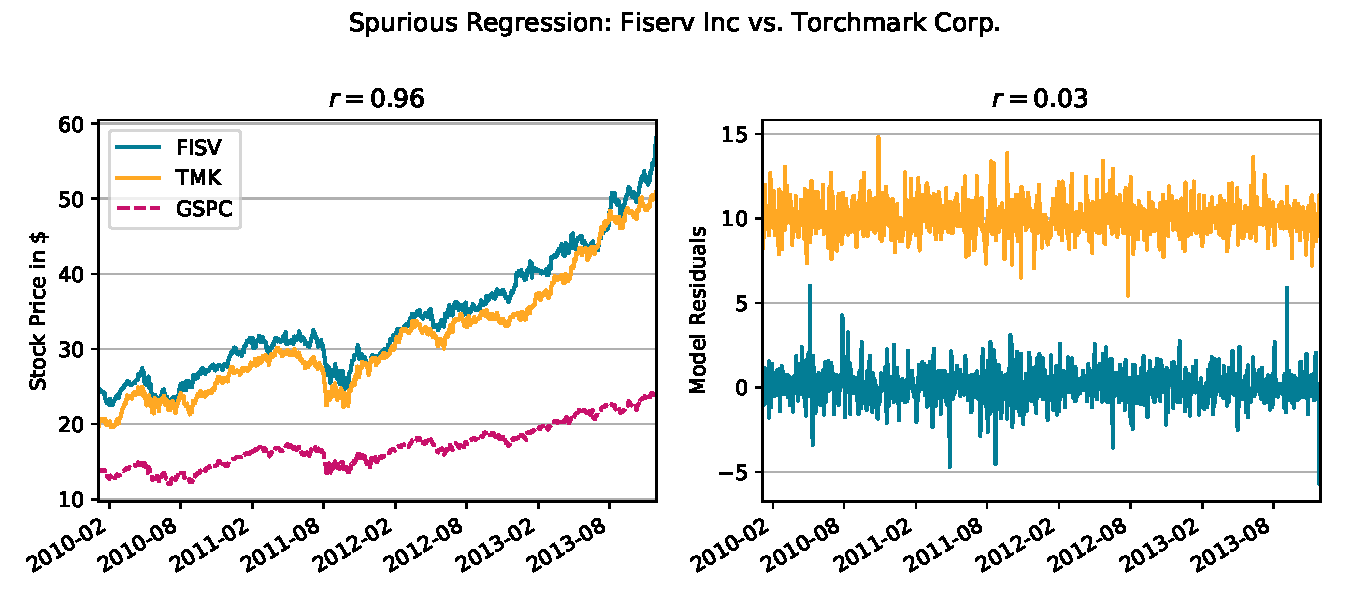
\includegraphics[width=\textwidth]{figures/regression/spurious-FISV-TMK.pdf}
    \caption{Data for the two companies \emph{Fiserv} and \emph{Torchmark}. The left plot shows the unmodified daily opening prices which revealed a Cross-Correlation of $r=0.99$. Additionally a scaled and shifted version of the market index is plotted. The right plot shows the same time series after properties like autocorrelation and heteroscedasticity were removed which led to $r=0.06$. For the sake of visibility, the orange time series is increased by 10.}
    \label{fig:spurious_regression}
\end{figure}

Even though $r$ is a very popular measure, it needs to be borne in mind that this measure does not account for nonlinear relationship which is not always a sufficient assumption. Therefore, the observed value might not fully reflect the real correlation but rather can be interpreted as an approximation. Since this limitation holds for all correlation values in this experiment, the values can fairly be compared to each other.

To see the impact of the several preprocessing steps, $r$ is calculated for each pair of stocks from four different phases. The distribution of $r$ for the original daily open prices, intraday returns, normalized returns and the residuals of the autoregressive models is visualized by violin plots in Figure~\ref{fig:steps-correlations-ind}. Because 467 stock prices are considered, there are 108.811 different pairs of stocks in total. With this high number of samples, the critical values for the 95~\% confidence interval are -0.006 and 0.006 respectively. Even for a more restrictive interval with $\alpha = 0.0001$, i.e. 99.99~\% confidence, the critical values are only -0.012 and 0.012 which for the whitened data in the last step still leads to 86~\% of all samples being significant. In consideration of this ever-present significance of correlation coefficients, the values are not evaluated by such confidence levels.

% Using the Student's $t$ distribution for the correlation coefficients

Except for autoregressive modelling, the distribution changes drastically with each preprocessing step. Initially, $r$ revealed a median of 0.48 and a great number of extreme values for the original stock prices. As the second distribution for price returns shows, this step does not tackle spurious correlation in a great manner. No pair of stocks is negatively correlated with each other since all stocks include the performance of the overall market or even the industry segment. After the exogenous impact was filtered out to a great extent, a more realistic distribution with a zero median can be observed. In general, stock prices share no more correlation with each other than the market performance and therefore reveal a coefficient close to zero. Relatively few stocks show a greater relationship which can be of a positive nature as well as of a negative nature.

\begin{figure}[!ht]
    \centering
    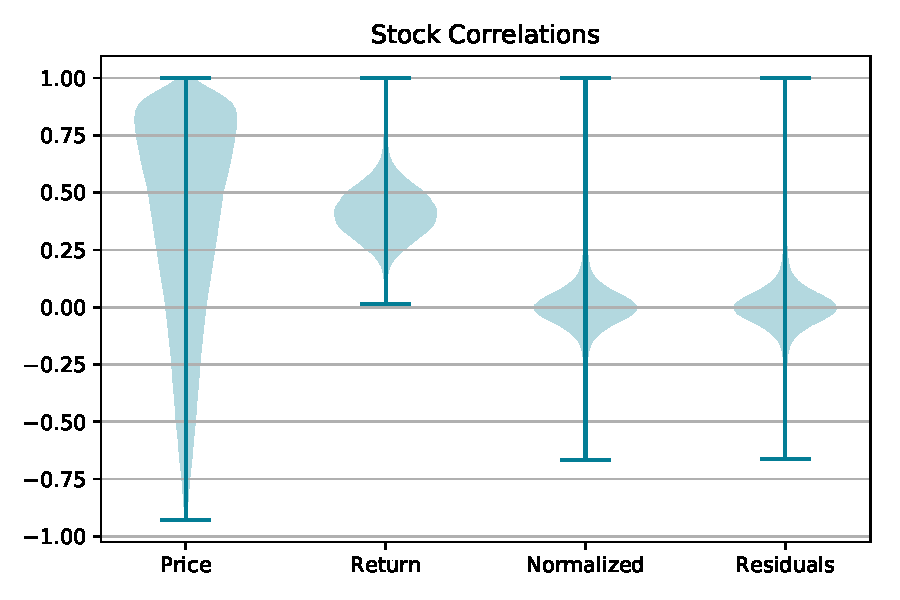
\includegraphics[width=0.8\textwidth]{figures/regression/steps-correlations-ind-norm.pdf}
    \caption{Violin plot of cross-correlation distributions for four main preprocessing steps. The filled area visualizes the approximated data distribution along the vertical line.}
    \label{fig:steps-correlations-ind}
\end{figure}

As mentioned in Section~\ref{subsubsection:processing:exogenous} the price returns can also be normalized by the S\&P~500 market index instead of separate industry means. For this alternative normalization method, the violin plots are shown in Figure~\ref{fig:steps-correlations-gspc}. Compared to the primary normalization by industry, the distribution is not located around zero but reveals a median of 0.2. Because all stocks are positively correlated with each other, this leads to the conclusion that not all exogenous influences are removed and therefore lead to spurious correlation. Concluding, the industry-wise normalization is preferable over market-wise normalization if one is interested in the cross-correlations among stocks from the same stock exchange.

\begin{figure}[!ht]
    \centering
    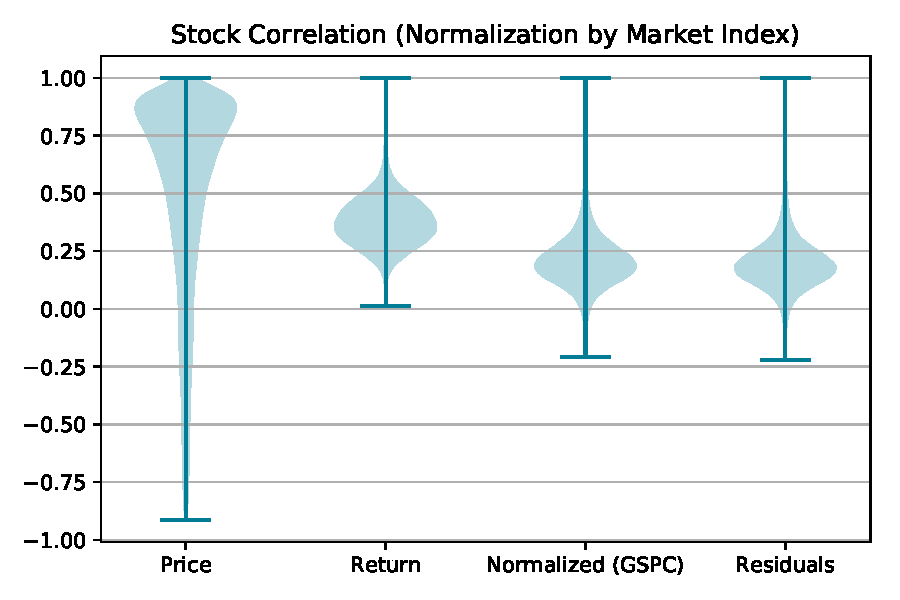
\includegraphics[width=0.8\textwidth]{figures/regression/steps-correlations-gspc-norm.pdf}
    \caption{Violin plot of cross-correlation distributions for four main preprocessing step with the normalization being adapted for market-wise instead of industry-wise normalization.}
    \label{fig:steps-correlations-gspc}
\end{figure}


\paragraph{Correlation Graph}

In order to visualize and inspect the calculated cross-correlations, a graph is defined and visualized in Figure~\ref{fig:graph-correlations}. As stated earlier in this section, there is a tremendous number of significant correlations. If all these correlations would be considered, the plotted graph would become unmanageable. Instead, the 99.9th percentile of all absolute correlation coefficients is calculated which equals 0.3688. Only positive or negative values outside of this percentile are considered for visualization. This leads to 109 correlations among 123 different stocks from all industry sectors. A node's size is determined respectively to its total revenue in 2010 in order to indicate its importance.

On this rather small and incomplete graph, individual nodes, connections and communities in the form of subgraphs can be further examined. It should be noted that the graph consists of the most extreme values and therefore is not a representative sample for the entire graph which would reveal an unmanageable number of edges.

\begin{figure}
    \centering
    \begin{subfigure}{\textwidth}
        \centering
        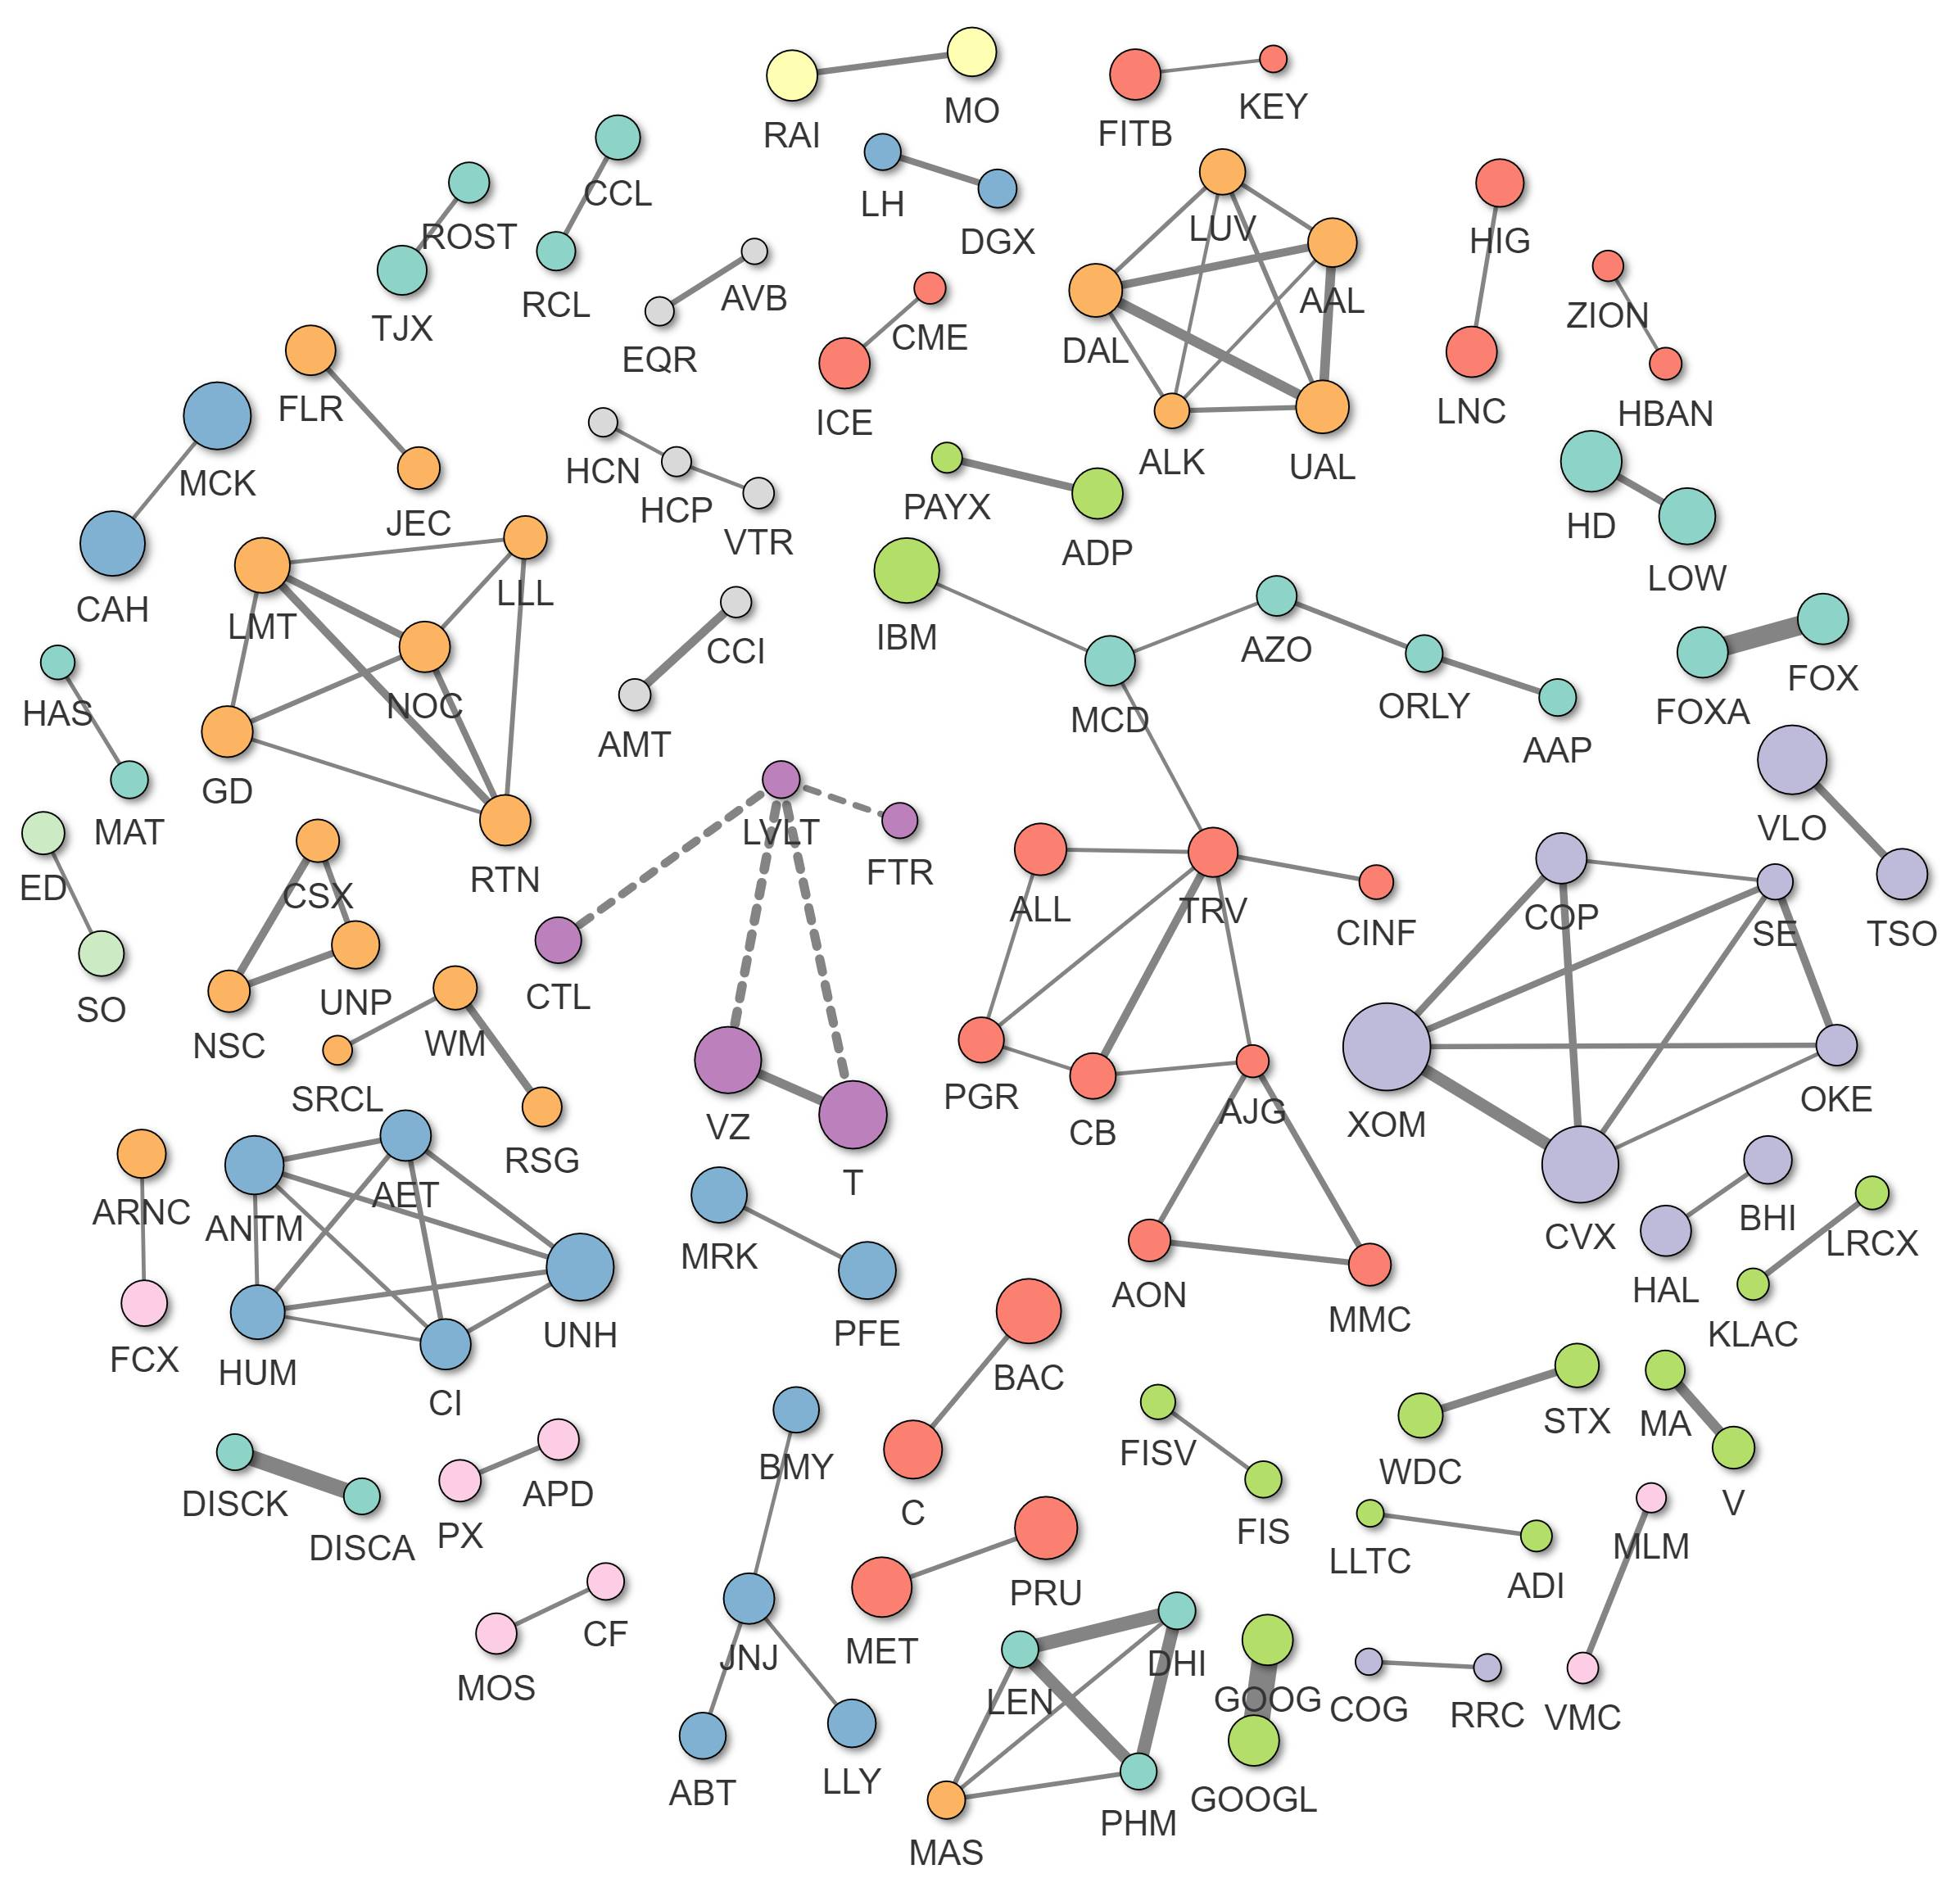
\includegraphics[width=\textwidth]{figures/regression/graph-corr-resid-999-42-with-neg.jpg}
    \end{subfigure}
    \vfill
    \begin{subfigure}{\textwidth}
        \centering
        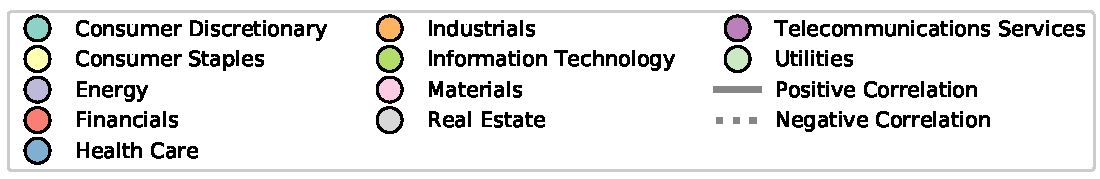
\includegraphics[width=\textwidth]{figures/graph-legend.pdf}
    \end{subfigure}

    \caption{Graph of the 109 greatest cross-correlations among stocks. Each node represents one stock which is labeled by the company's ticker symbol and coloured by the regarding industry section. Which color belongs to which industry is provided by the legend below. The node's size is determined by the total revenue for this company. Each edge between two nodes represents the cross-correlation $r$ between those stocks. More extreme values are indicated by a thicker edge and negative values by a dashed line.}
    \label{fig:graph-correlations}
\end{figure}

As indicated by the node colors, a large proportion of high correlations are observed among companies belonging to the same industry sectors. Only eight edges between two different sectors are present in this visualization. In terms of inter-industry connections, the node \emph{MCD} (\emph{McDonald's Corp.}) in the center of the graph is the strongest one since it is connected to nodes from three different industries. Investigation by financial news did not reveal an underlying relationship with the connected companies. Instead, this stock appears to be an appropriate strong representative component of the market performance and therefore is strongly linked to other important representative components like \emph{IBM} (\emph{International Business Machines}).

From the 109 edges selected for the graph, only four represent a negative correlation which all originate from the industry sector \emph{Telecommunications Services}. Further, it should be noted that there a three companies for which each one compromises two stocks. The reasoning for this is given in the previous Section~\ref{section:data}. Because two stocks of the same company are almost equal. these three correlation pairs reveal the highest $r$.

As denoted previously, this graph is not representative for the meaning of the measured cross-correlations. In order to examine this feature's usability, the final evaluation in Section~\ref{section:evaluation} will conduct a comparison with the extracted business relationships which are introduced in the following section.




% \begin{itemize}
%     \item Describe graph figure. Which correlation where chosen (99.9~\% Percentile: 0.3688, 123 nodes, 109 edges (incl 4 neg), 11 industries)
%     \item Collect insights: Only 8 edges between comps with different industry. Concluding, industry-correlation still exists
%     \item Not whole industries are connected but only pairs within industries giving evidence more meaningful relationships than just being in the same industry.
%     \item \emph{McDonald's Corp.} (node \emph{MCD} in the center of the graph) is the strongest connected node across several industries. Since investigation did not reveal an underlying relationship with the connected companies, this stocks instead appears to be an appropriate strong representative component of the market performance.
%     \item{Pairs of two stocks belonging to the same company are not removed}
% \end{itemize}




% \todo{Optional: Mutual Information, Cointegration, Granger Causality}

%%% Inspecting Cross-Dependencies
% Look into Dean2015 for more insights
% Calculate cross-correlation between residuals of stocks.
% Visually inspect change of cross-correlations over years? (like Mantegna)
% -> Inspect normalized MI and Pearson's r (as done by Dionisio)

% Cointegration & Causality Analysis
% Paper using Cointegration (Johansen Test): Kosapattarapim2017 https://drive.google.com/file/d/1wMcZlYGR69HT-JAH5382FIyfS4yh5gCC/view
% Paper using Granger Causality: Bollean2011 https://drive.google.com/file/d/1hv6CoM-_GnhDtVOGjhu-N3btCAIaA1an/view
% BDS (Bock, Dechert and Scheinkman[Hsieh 1989]) test (Dionisio2004) to test if variables are nonlinear independent
% Test for Unit Root, Cointegration, Granger Causality (bidir gc vs. simultaneity)



% Inspect correlation and prices in general for one specific quarter (e.g. 2011/02 appears to be bad for Energy)




% Prediction:

% For experiments incorporating both datasets only the overlapping time period is used. Training: 2010 - 2013 (1st half), Test: 2013 (2nd half). Test is left out up to the final evaluation. The training set will be splitted into chunks to apply cross-validation (as pointed out by Hsu et al) along time series (e.g. Li et al 2014).
% How to upsample stock prices?
% Stratified sampling to ensure similar class distribution in train, val & test ?
% Evaluate good class threshold
% Evaluate good prediction frame size



%%% Links Stack
% Links about regression steps
% Example 1: Regression Diag http://songhuiming.github.io/pages/2016/12/31/linear-regression-in-python-chapter-2/
% Example 2: Regression Diag https://www.statsmodels.org/0.8.0/examples/notebooks/generated/regression_diagnostics.html
% Example: ARIMA & GARCH modelling http://www.blackarbs.com/blog/time-series-analysis-in-python-linear-models-to-garch/11/1/2016
% Example 3: Testing for Unit root and cointegration
% https://pdfs.semanticscholar.org/7ce6/2a0c7f6dab85f264a5403bf9b99a0f20a156.pdf
% Example: Apply ARMIA vs GARCH  https://scialert.net/fulltextmobile/?doi=jas.2011.1129.1135
% Methodology for ARIMA, GARCH, etc.: https://sci-hub.se/10.2139/ssrn.2540535
% Example 1: Regression Model https://www.kaggle.com/benjibb/prototype-gspc


\section{Text Analysis}
\label{section:text_analysis}
Besides stock prices, financial news can also be used as a proxy for business relationship. If an announcement was made or any relevant information like a SEC filing was released by a company, financial news report it as fast as possible. Longer reports put it even into a bigger picture, provide some background information and refer to possible competitors. Two companies are most likely mentioned together in the same article, if they are related to each other in any context. The simultaneous mentioning of two companies within one article is called co-occurrence in the following.

\subsection{Named Entity Recognition}

Before collecting co-occurrences, first the occurrence of each company needs to be extracted and linked separately. If an author is writing news, there are many problems for determining whether, and if so which, companies are the topical subject. He might use an alias name, a product of the company (e.g. \emph{Google} instead of \emph{Alphabet}) or just a representative like the CEO (e.g. \emph{Steve Jobs} instead of \emph{Apple}). As a first heuristic approach, only the occurrences of company names are considered. After applying NER on the corpus of financial news \footnote{Implementation by SpaCy: https://spacy.io}, all entities which are labeled as organizations like companies, agencies or institutions are collected. This results in 9.6 out of 40.7 million entities.

%  \todo{mention example (use elasticsearch)}
% \todo{Example snippet of news with different tagged organizations (and other tags}
% https://spacy.io/api/annotation#named-entities

% This requires to recognize corporation names which might be tackled using Named Entity Recognition (NER) or even more complex approaches as the algorithms by Rau \cite{Rau1991:extractNames} or Loster et al. \cite{Loster2017:comp_rec}.

\begin{figure}
    \centering
    \frame{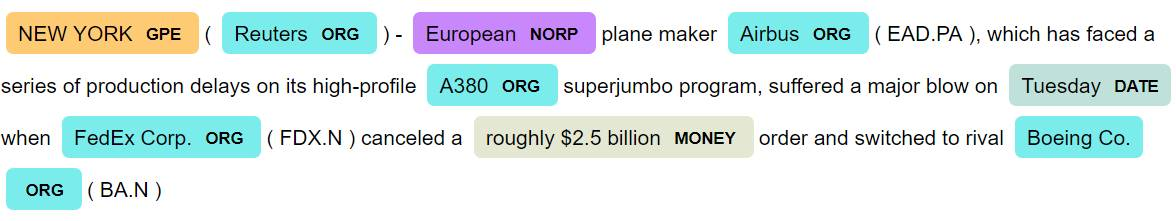
\includegraphics[width=\textwidth]{figures/text/entities-displacy.jpg}}
    \caption{Classified entities for the Reuters article \enquote{FedEx cancels Airbus A380 order, switches to Boeing} (2006-11-07). Each of the five entity types is marked by another color whereas organization are lightblue. An abbreviation of each label is added behind the labeled sequence in bold letters. For example, NORP represents nationalities among others and ORG represents companies, institutions, etc. The content reports a policy change by \emph{FedEx Corporation} in favour of \emph{Boeing Company}.} 
    \label{fig:ner-entities}
\end{figure}

To give an example, how a financial news article and extracted entities might look like, Figure~\ref{fig:ner-entities} shows a selected section in a Reuters article from the 7th of November, 2006. Although, the aircraft \emph{A380} is falsely recognized as an organization, the four mentioned companies are correctly tagged. One might note that in this example, stock symbols are already provided in brackets within the text. Even though, they can be used to set up a link between company and stock price, such additional information are often missing in the examined text-corpus. How these tagged organizations are automatically linked to companies on the stock market and thereby to the regarding stock prices, will be shown in the next section.


\subsection{Named Entity Linking}

Out of all organization entities, only those are of interest which can be linked to a company from the S\&P~500 market index. The official company name is provided by the stock dataset and linked to the correct stock prices by its stock symbol. The names contain unhandy suffixes like \emph{Inc.} or \emph{Limited} which are usually left out in the news. To establish the link between occurrences in news and the full corporate name, a regular expression is used to remove the name extensions from both values:

\DefineShortVerb{\!}
\SaveVerb{VerbA}! ,?[^\w](Corp\ A|A\ Corp|\&\ Co|Svc\.Gp| !
\SaveVerb{VerbB}! Corp(?:oration|'s)?|Inc|Co(?:s|mpany)?| !
\SaveVerb{VerbC}! Ltd|Limited|Plc|Group|(?:International| !
\SaveVerb{VerbD}! Int'l)(?:\ Inc)?|Int'l\ Industries)\.?$ !

\begin{align}
  \begin{split}
    \UseVerb{VerbA} \\ \UseVerb{VerbB} \\ \UseVerb{VerbC} \\ \UseVerb{VerbD}
  \end{split}
  \label{formula:linking_regex}  \\ \eqname{Regular Expression}
\end{align}

% After the suffices are removed from both sides, the remaining strings are not safely matching. To allow small deviations a fuzzy matching metric, namely the Damerau–Levenshtein distance \cite{Damerau1964}, is applied. It measures the edit distance between two strings considering the insertion, deletion, substitution and transposition of characters.

If the regular expression reduced both strings to their least common sequence and they are completely equal, the extracted entity is assumed to match the examined stock company. In the end, 436.000 related company names were extracted which are distributed over 127.000 articles. Because occurrences were only found for 443 companies, the remaining companies are removed in the remainder of this study.

\begin{figure}
    \centering
    \frame{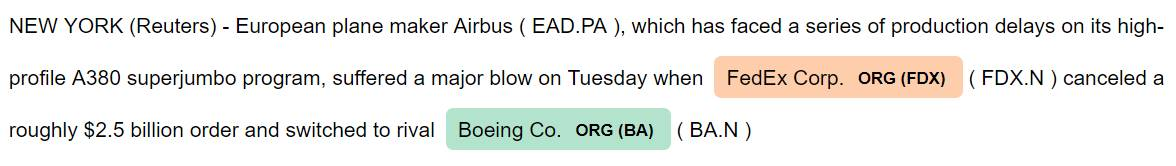
\includegraphics[width=\textwidth]{figures/text/entities-displacy-org.jpg}}
    \caption{Linked companies for the same article as in Figure~\ref{fig:ner-entities}. Hereby, the colors are differing for each linked company. To indicate the established link, the bold tag behind the labeled sequence contains the regarding stock symbol.}
    \label{fig:ner-entities-org}
\end{figure}

Figure~\ref{fig:ner-entities-org} shows the same financial news article as before but highlights occurrences of linked company only. Two of four companies are linked to stock prices, whereas the remaining two are not considered since they are not components of the market index and thereby not contained by the data covered in this work.

\subsection{Co-occurrence Features}

To measure the relationship between two companies based on these occurrences, a feature needs to be found. Therefore, three different approaches are proposed:
% \begin{enumerate*}[label=(\roman*)]
%     \item Co-occurrences;
%     \item Minimum Distance;
%     \item Pairwise Distance
% \end{enumerate*}.
% https://arxiv.org/pdf/1506.07220.pdf

\begin{enumerate}[
leftmargin=0pt, itemindent=20pt,
labelwidth=15pt, labelsep=5pt, listparindent=0.7cm,
align=left, label={\textbf{(\arabic*)}}]
\item \textbf{Co-occurrences} of two companies is calculated by the number of articles in which both company names occur. If this is the case, the article is likely to write something about their business relationship. This feature does not account for the number or distance of occurrences for one company within one article. It rather measures the co-occurrences across the whole text corpus instead of weighting the connection within one article.
\item \textbf{Minimum Distance} takes the intra-article connection into account by calculating the distance for each possible pair of company names within one article. Subsequently, the smallest possible distance is kept for this article. The distance between two entities is represented by the starting indices of the initially matched string. To unite the article-wise values, all minimum distances across all articles are averaged. If two companies are strongly connected, authors are more likely to provide comparisons between them. This will be reflected by an average smaller distance for co-occurrences of two companies across all articles.
\item \textbf{Pairwise Distance} is a more sophisticated approach compared to the previous ones. It accounts for the multiple inter-article co-occurrences as well as the multiple intra-article co-occurrences. Therefore, a scan line algorithm will traverse all occurrences of these two companies in an article and pair these up while avoiding a too high distance. Similar to the previous approach, all distances are averaged but, in addition, each pair is considered instead of only considering the best one for each article.
\end{enumerate}

For these three features the suitability will be evaluated in the next section when they are compared to the previously generated stock price correlations. To provide a first examination of text-based features in general, a graph is shown in Figure~\ref{fig:graph-cooccurrence-pairwise} which was generated in the same fashion as previously done for the cross-correlations among prewhitened stock prices. The strength of edges is calculated by their pairwise distance across the whole news corpus. Because there are 15.184 pairs with a non-zero pairwise distance, all values below the 99.9th percentile are left out. This resulted in 90 edges between 98 nodes from all eleven industry sectors. As already stated in respect to the previous graph, the graph consists of the most extreme values and therefore is not a representative sample for the entire graph.

% 0.994, 0.4985 with people and halved

\begin{figure}
    \centering
    \begin{subfigure}[b]{\textwidth}
        \centering
        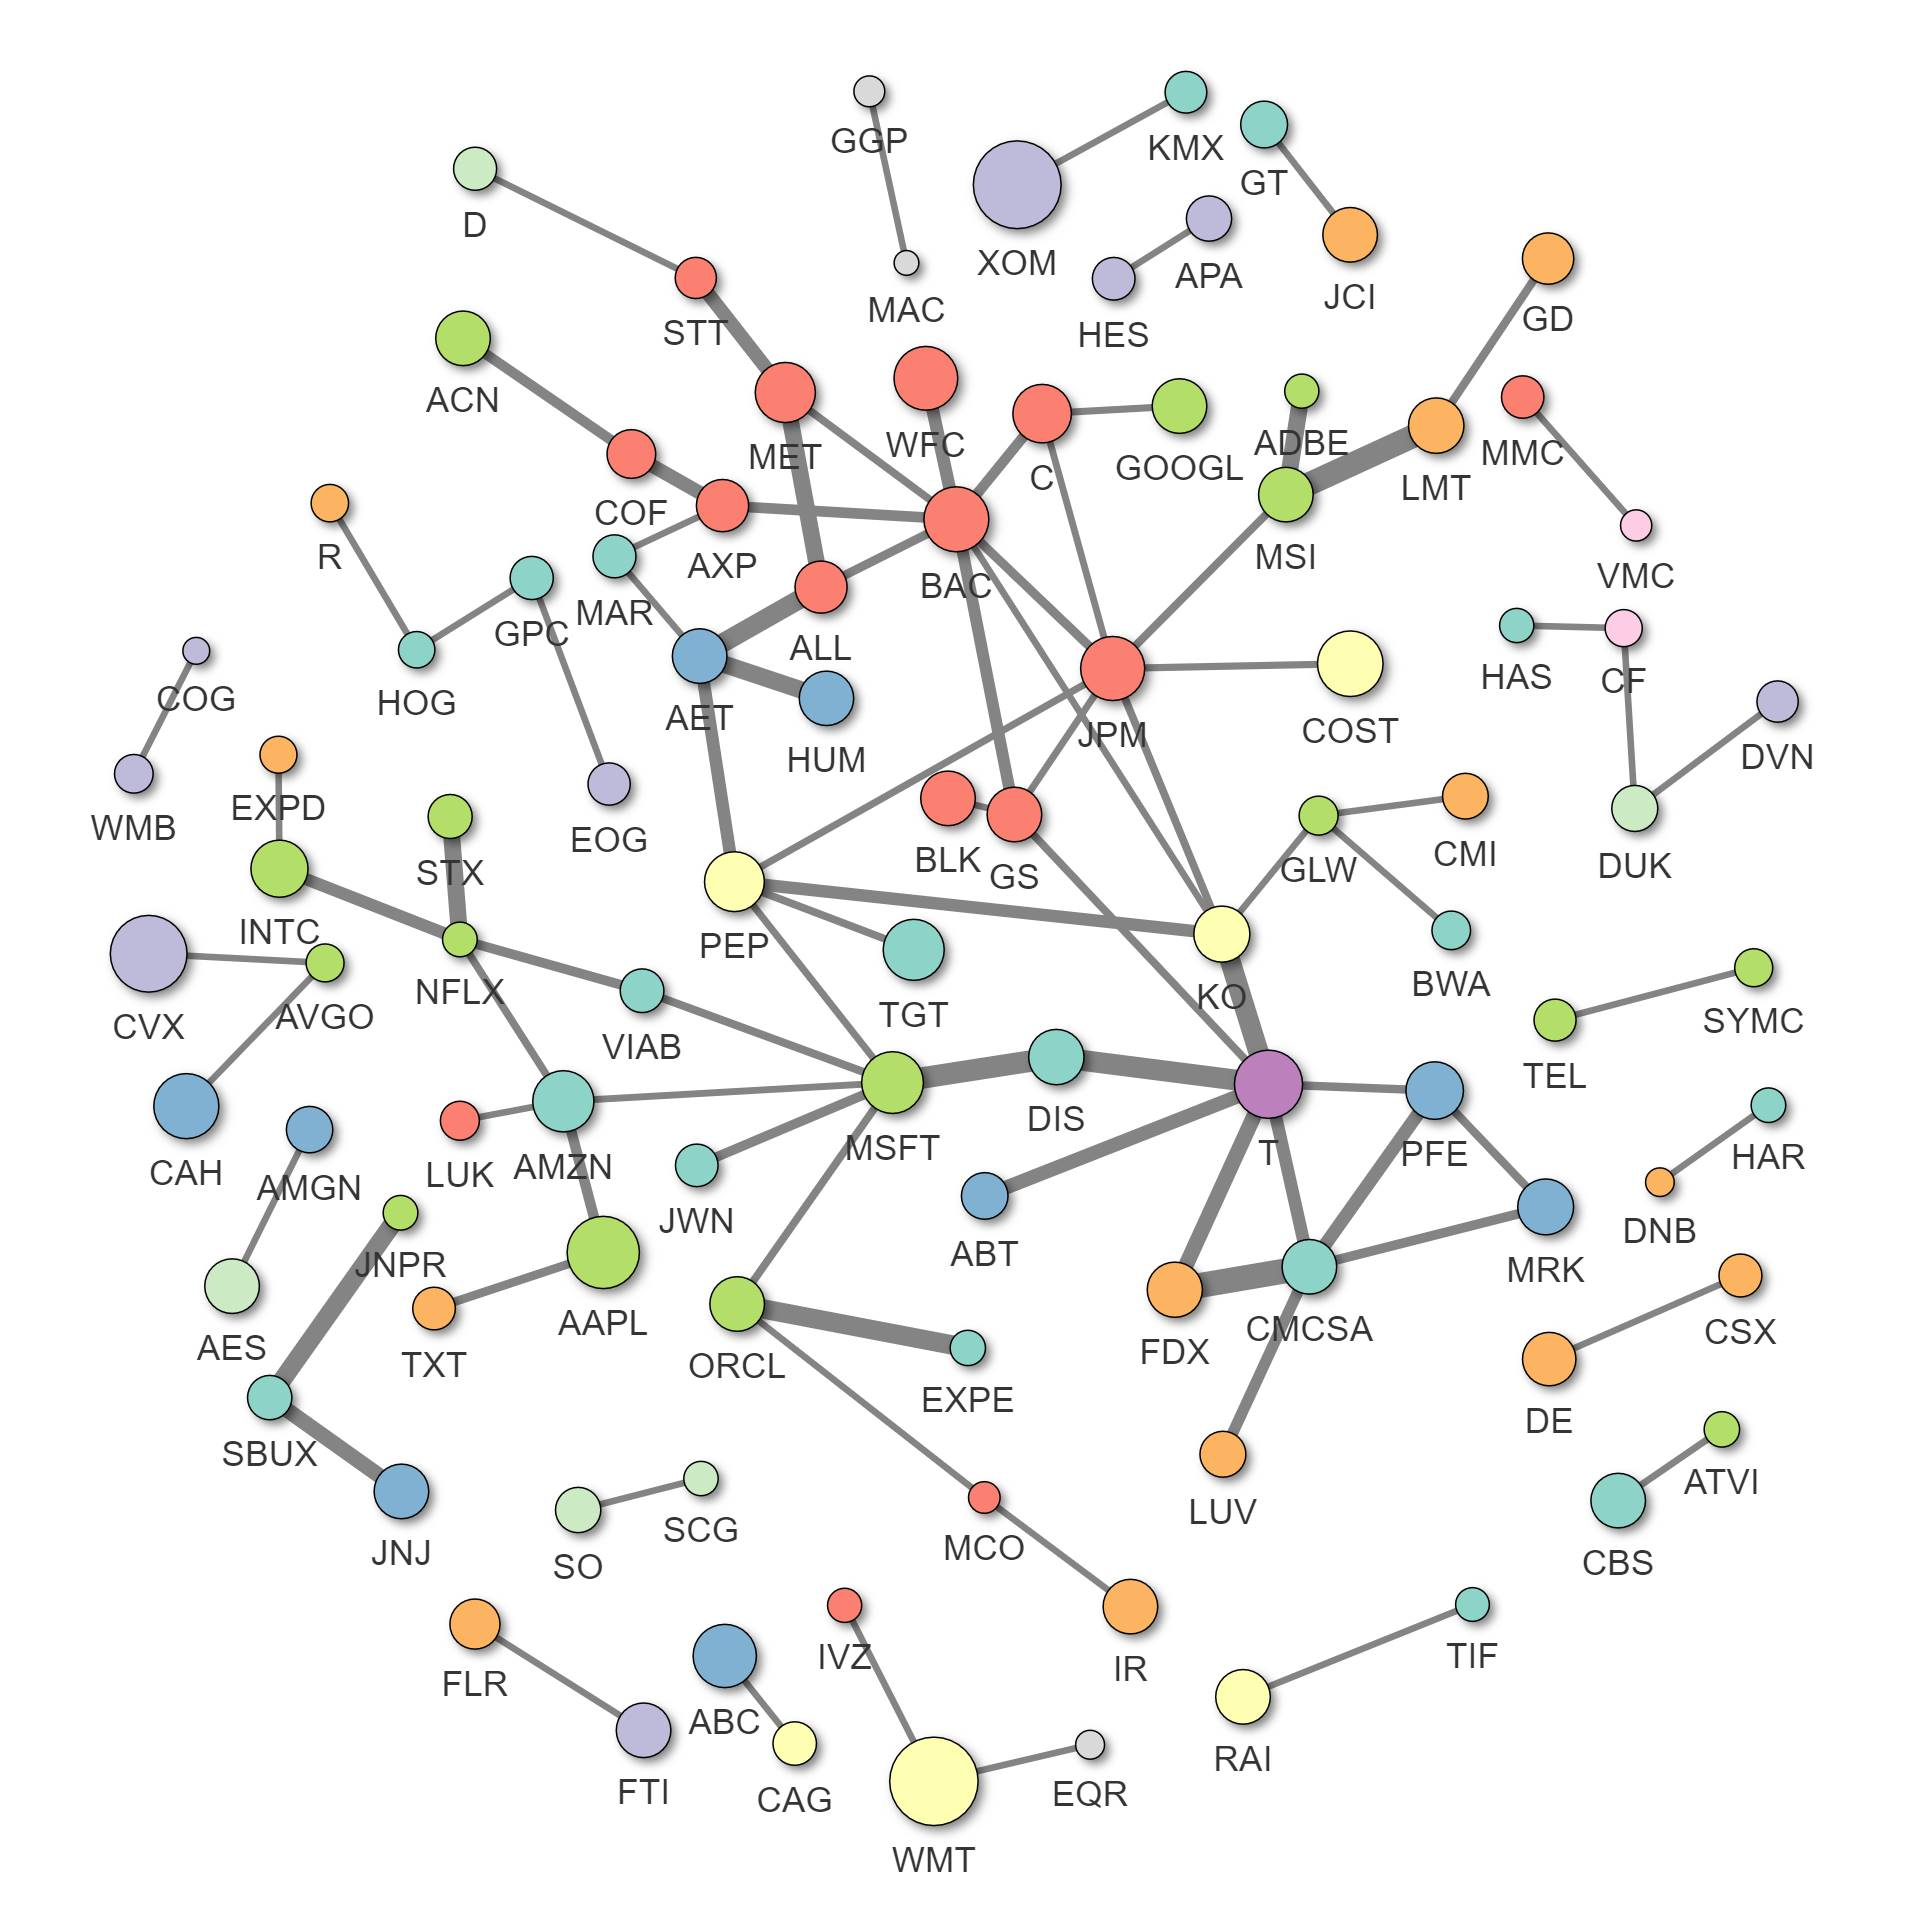
\includegraphics[width=\textwidth]{figures/text/graph-pair-dist-999-42.jpg}
    \end{subfigure}
    \vfill
    \begin{subfigure}[b]{\textwidth}
        \centering
        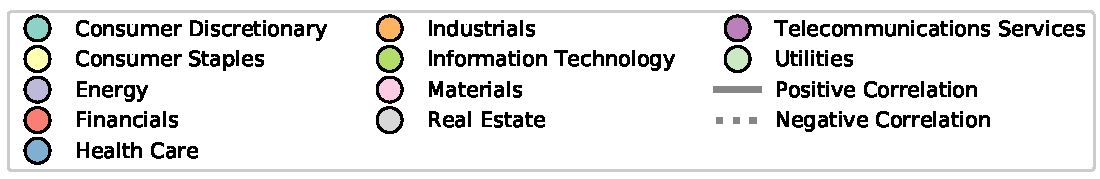
\includegraphics[width=\textwidth]{figures/graph-legend.pdf}
    \end{subfigure}

    \caption{Graph of the 90 strongest connections, measured by the calculated pairwise distance among two companies. Each node represents one company which is labeled by the companies ticker symbol and coloured by the regarding industry section. Which color belongs to which industry is provided by the legend below. The node's size is determined by the total revenue for this company. Each edge between two nodes represents the pairwise distance between the co-occurrences of the regarding companies. More extreme values are indicated by a thicker edge.}
    \label{fig:graph-cooccurrence-pairwise}
\end{figure}

Compared to the correlation graph in Figure~\ref{fig:graph-correlations}, this one reveals a very different structure. Both graphs share 29 nodes and four edges only. Instead of many small decoupled subgraphs for industry sectors this graph reveals one big subgraph consisting of 50 nodes from many different industry sectors. Some edges between companies sound comprehensible after investigating their business relationships. For example, \emph{Microsoft Corp.} (\emph{MSFT}) and \emph{Viacom Inc.} announced a long-term strategic alliance for corporate segments like game development and advertisement in 2007. To mention another example, a high pairwise distance can be observed for both streaming providers \emph{Netflix Inc.} (\emph{NFLX}) and \emph{Amazon.com Inc.} (\emph{AMZN}) which both benefit from the increased demand in this segment of the market.

Over the whole graph, only 28 edges are connections among companies originating from the same industry. The greatest industry cluster can be observed for companies from the sector \emph{Financials} which includes insurance companies (e.g. \emph{American International Group, Inc.}), investment banks (e.g. \emph{JPMorgan Chase \& Co.}) and financial service providers (e.g. \emph{Citigroup Inc.}). Some of them are densely connected with other industries which can be argued by their investments in stocks of other companies.


% No stock prices between 2006 and 2010. Check if the features extracted from this span is relevant.

% Word Embedding Distance
% General Embedding
% Domain-based

% Co-Mentioning Network from News text: https://link.springer.com/chapter/10.1007/978-3-319-92871-5_7


% Prediction
% Averaged Word Vectors vs. Tfidf Vectors	
% Most common words during up/down
% Sentiment vs Price Movement
%   For further analyses drop all entities from text

% \missingfigure[figwidth=6cm]{Testing a long text string}

\section{Evaluation}
\label{section:evaluation}
Until this point, features from two different datasets were extracted which might be related to business relationships. Unfortunately, there are no true labels available for validating the features suitability. Instead, the features from both types of data are compared to each other. Since they are both considered to be, at least, related to the latent variable, namely the business relationship, a correlation should be observable.

For measuring bivariate correlation, there are several approaches established. As mentioned earlier in this work, Pearson's $r$ is among the most popular ones. Even though it is a very common metric, it only considers a linear relationship. Since this evaluation covers non-temporal variables which share no common data source, spurious correlation is assumed to be not present or have a negligible impact.

To account for nonlinear monotonic relationships and get more robust results on non-normal, skewed or heteroscedastic data, a rank-based correlation like Spearman's $\rho$ or Kendall's $\tau$ is recommended \cite{Kowalski1972OnCoefficient}. The latter is generally preferred since it has a lower gross-error-sensitivity \cite{Croux2010InfluenceMeasures} and therefore offers a more robust estimation of the underlying population with more reliable confidence intervals \cite{Newson2002ParametersDifferences}. In the following, $r$ and $\tau$ are examined for the stock correlation from Section~\ref{section:statistical_analysis} and the three extracted news feature from Section~\ref{section:text_analysis}. As an comparable heuristic, a dichotomous feature called \textbf{Same Industry} is added. It equals one if a pair of companies originated from the same industry, otherwise it equals zero.

Because the news reveal occurrences for 443 companies and stock prices were available for 467 companies, only those were considered for which both co-occurrences and stock price correlation could be generated. This resulted in 417 companies and 86.736 unique bidirectional pairs.

In the following two experiments will be conducted. At first, the three news-based features for co-occurrence are correlated with the stock cross-correlations to find out, which is to be the most suitable one. Subsequently in the second experiment, the most promising news-based feature is compared with the intermediate preprocessing steps for the stock prices in order to evaluate if they are supportive for a higher correlation with co-occurrence.

Because all co-occurrence features consider the presence of a relationship without describing its semantic, they can not be directly correlated with the stock correlations. Instead, the stock correlation will be adjusted by taking their absolute value. Hence, they do not account for negative relationships either.

% https://stats.stackexchange.com/questions/8071/how-to-choose-between-pearson-and-spearman-correlation
% https://stats.stackexchange.com/questions/3730/pearsons-or-spearmans-correlation-with-non-normal-data


\subsection{Text-based Features}
\label{subsection:evaluate_text_features}

\begin{table*}
    \centering
    \setlength{\tabcolsep}{0pt} % Default value: 6pt
    
    \begin{tabular*}{0.8\textwidth}{@{\extracolsep{\fill}}cccc}
        \toprule
        {} &  Stock Correlation &  Same Industry \\
        \midrule
        \textbf{Co-occurrences}     & 0.0799 & 0.0690 \\
        \textbf{Minimum Distance}   & 0.0947 & 0.1477 \\
        \textbf{Pairwise Distance}  & \textbf{0.1105} & \textbf{0.1643} \\
        \bottomrule
    \end{tabular*}
    
    \caption{Pearson's $r$ for the three text-based features \emph{Co-occurrences}, \emph{Minimum Distance} and \emph{Pairwise Distance}, compared with the \emph{Stock Correlation} and the heuristic \emph{Same Industry}.}
    \label{table:corr-text-r}
\end{table*}

% {} &  Stock Corr. &  Co-occurrences &  Min. Dist. &  Pairwise Dist. &  Industry \\
% \midrule
% \textbf{Stock Corr.}       & 1.0000 & 0.0799 & 0.0947 & 0.1105 & 0.2013 \\
% \textbf{Co-occurrences}    & 0.0799 & 1.0000 & 0.1594 & 0.1635 & 0.0690 \\
% \textbf{Min. Dist.}        & 0.0947 & 0.1594 & 1.0000 & 0.8622 & 0.1477 \\
% \textbf{Pairwise Dist.}    & 0.1105 & 0.1635 & 0.8622 & 1.0000 & 0.1643 \\
% \textbf{Industry}          & 0.2013 & 0.0690 & 0.1477 & 0.1643 & 1.0000 \\

The three features extracted from news, namely \textbf{Co-occurrences}, \textbf{Minimum Distance}, \textbf{Pairwise Distance}, are compared with the stock correlations calculated on the price residuals which are considered to be the most stable data and free of autoregressive properties. Pearson's $r$ for the text-based features, stock correlation and the industry feature is reported in Table~\ref{table:corr-text-r}. Compared with the stock correlation, all three text-based features reveal a highly significant linear correlation exceeding the 99~\% confidence interval. The distance based approaches are superior to the plain co-occurrences features. The pure co-occurrences features might be affected by the selection of news topics, leading to small values for sparsely occurring but important companies. The other two features do not account for the overall number of mentions but only rate the average distance between entities of two companies. This leads to the supposition that the frequency is less important than the intensity of co-occurrences for describing the relationship of two companies. The highest correlation is observed for the more sophisticated approach, the pairwise distance, which might be caused by the higher number of accounted co-occurrences and therefore leads to a higher precision.

\begin{table*}
    \centering
    \setlength{\tabcolsep}{0pt} % Default value: 6pt
    
    \begin{tabular*}{0.8\textwidth}{@{\extracolsep{\fill}}cccc}
        \toprule
        {} &  Stock Correlation &  Same Industry \\
        \midrule
        \textbf{Co-occurrences}    & \textbf{0.0505} & 0.1431 \\
        \textbf{Min. Dist.}        & 0.0479 & 0.1377 \\
        \textbf{Pairwise Dist.}    & 0.0497 & \textbf{0.1435} \\
        \bottomrule
    \end{tabular*}
    
    \caption{Kendall's $\tau$ for the three text-based features \emph{Co-occurrences}, \emph{Minimum Distance} and \emph{Pairwise Distance}, compared with the \emph{Stock Correlation} and the heuristic \emph{Same Industry}.}
    \label{table:corr-text-tau}
\end{table*}


% {} &  Stock Corr. &  Co-occurrences &  Min. Dist. &  Pairwise Dist. &  Industry \\
% \midrule
% \textbf{Stock Corr.}       & 1.0000 & 0.0505 & 0.0479 & 0.0497 & 0.1213 \\
% \textbf{Co-occurrences}    & 0.0505 & 1.0000 & 0.9118 & 0.9349 & 0.1431 \\
% \textbf{Min. Dist.}        & 0.0479 & 0.9118 & 1.0000 & 0.9591 & 0.1377 \\
% \textbf{Pairwise Dist.}    & 0.0497 & 0.9349 & 0.9591 & 1.0000 & 0.1435 \\
% \textbf{Industry}          & 0.1213 & 0.1431 & 0.1377 & 0.1435 & 1.0000 \\

The monotonic relationship measured by the rank-based coefficient Kendall's $\tau$ is shown in Table~\ref{table:corr-text-tau}. Measured upon presence of correlation, $\tau$ is considered to be more restrictive which can be observed for all three text-based features compared to stock correlation. The advantage of using ranked variables instead of absolute values can be observed for the correlation between both features industry and co-occurrences. Both rely on integer values and thus interfere the correlation coefficient measured by $r$ which assumes continuous variables.

Contradictory to the previous findings based on $r$, there is no great difference between the three text-based approaches for $\tau$. The discrepancies might be caused by $\tau$ considering any kind of monotonic relationship but putting less focus on an actual plain linear relationships. However, it raises doubts about whether the distance based measures are actually superior and whether the pairwise distance is the most promising approach. Nevertheless, all three correlations are again significant with 99~\% confidence and therefore valuable features for reflecting business relationships.

\subsection{Stock Correlations}

For retrospectively inspecting the impact of preprocessing steps on the stock prices, the pairwise distance is compared with each preprocessing step in Table~\ref{table:corr-stock-r}. It should be noted that all stock correlations except for the one based upon model residuals are prone to spurious correlation and therefore need to be treated with caution.

\begin{table*}
    \centering
    \setlength{\tabcolsep}{0pt} % Default value: 6pt
    
    \begin{tabular*}{0.8\textwidth}{@{\extracolsep{\fill}}cccc}
        \toprule
        {} &  Pairwise Distance &  Same Industry \\
        \midrule
        \textbf{Price}        & -0.0131 & 0.0553 \\
        \textbf{Return}       &  0.0936 & \textbf{0.2679} \\
        \textbf{Normalized}   &  0.1091 & 0.1963 \\
        \textbf{Residuals}    &  \textbf{0.1105} & 0.2013 \\
        \bottomrule
    \end{tabular*}
    
    \captionsetup{singlelinecheck=off}
    \caption[foo bar]{Pearson's $r$ for the \emph{Pairwise Distance} and the heuristic \emph{Same Industry}, compared with the stock correlation based on the data from intermediate preprocessing steps: \begin{enumerate*}[label=(\roman*)]
        \item original price
        \item intraday returns
        \item industry-wise normalized returns
        \item residuals from autoregressive models
    \end{enumerate*}.}
    \label{table:corr-stock-r}
\end{table*}

% {} &  Distance &   Price &  Return &  Normalized &  Residuals &  Industry \\
% \midrule
% \textbf{Distance}          &  1.0000 & -0.0131 &  0.0936 & 0.1091 & 0.1105 & 0.1643 \\
% \textbf{Price}             & -0.0131 &  1.0000 &  0.1783 & 0.0418 & 0.0398 & 0.0553 \\
% \textbf{Return}            &  0.0936 &  0.1783 &  1.0000 & 0.1296 & 0.1299 & 0.2679 \\
% \textbf{Normalized}        &  0.1091 &  0.0418 &  0.1296 & 1.0000 & 0.9882 & 0.1963 \\
% \textbf{Residuals}         &  0.1105 &  0.0398 &  0.1299 & 0.9882 & 1.0000 & 0.2013 \\
% \textbf{Industry}          &  0.1643 &  0.0553 &  0.2679 & 0.1963 & 0.2013 & 1.0000 \\

As one might expect, no significant relationship can be observed based upon original stock prices. After taking the daily returns, the relationship is present justifying this step. Considering $r$, the relationship again increases after industry-wise normalization and taking the residuals from autoregressive models. Although industry affiliation appears to be highly correlated with the pairwise distance, the stock correlation increases after this factor is assumed to be removed.

\begin{table*}
    \centering
    \setlength{\tabcolsep}{0pt} % Default value: 6pt
    
    \begin{tabular*}{0.8\textwidth}{@{\extracolsep{\fill}}cccc}
        \toprule
        {} &  Pairwise Distance  &  Same Industry \\
        \midrule
        \textbf{Price}       & -0.0309 & 0.0456 \\
        \textbf{Return}      &  0.0480 & \textbf{0.1876} \\
        \textbf{Normalized}  &  0.0496 & 0.1195 \\
        \textbf{Residuals}   &  \textbf{0.0497} & 0.1213 \\
        \bottomrule
    \end{tabular*}
    
    \captionsetup{singlelinecheck=off}
    \caption[foo bar]{Kendall's $\tau$ or the \emph{Pairwise Distance} and the heuristic \emph{Same Industry}, compared with the stock correlation based on the data from intermediate preprocessing steps: \begin{enumerate*}[label=(\roman*)]
        \item original price
        \item intraday returns
        \item industry-wise normalized returns
        \item residuals from autoregressive models
    \end{enumerate*}.}
    \label{table:corr-stock-tau}
\end{table*}


% {} &  Distance &   Price &  Return &  Normalized &  Residuals &  Industry \\
% \midrule
% \textbf{Distance}    &  1.0000 & -0.0309 &  0.0480 & 0.0496 & 0.0497 &    0.1435 \\
% \textbf{Price}       & -0.0309 &  1.0000 &  0.1127 & 0.0186 & 0.0176 &    0.0456 \\
% \textbf{Return}      &  0.0480 &  0.1127 &  1.0000 & 0.0570 & 0.0564 &    0.1876 \\
% \textbf{Normalized}  &  0.0496 &  0.0186 &  0.0570 & 1.0000 & 0.8735 &    0.1195 \\
% \textbf{Residuals}   &  0.0497 &  0.0176 &  0.0564 & 0.8735 & 1.0000 &    0.1213 \\
% \textbf{Industry}    &  0.1435 &  0.0456 &  0.1876 & 0.1195 & 0.1213 &    1.0000 \\

Even the more conservative correlation coefficients for $\tau$ in Table~\ref{table:corr-stock-tau} show an increase of correlation throughout all preprocessing steps. For the original stock price, a negative correlation with the pairwise distance can be observed. As shown in earlier in this work, correlation based on these values reveal large spurious correlation which make further evaluation on them neglectable. Hence, the observation of a negative relationship between stock correlation and business relationship is not supported.


\subsection{Period of Comparison}
As pointed out previously in Section~\ref{section:data}, the selected time periods from both considered datasets do not match. Because the relationship extracted from news are expected to have a long-term impact, the text-based features are generated from 2006 until 2013 while the stock correlations are generated on historical prices from the last four years only. To inspect the impact of this decision, all text-based features were recalculated for the same period as for the stock prices. Though the values for $r$ from the previous tables did increase by a few thousandths, the difference is very small and therefore considered to be not significant. This might be justified by the fact that a majority of articles is distributed over the same four years as the historical stock prices.

\subsection{Discussion}

In the first part of analysis, namely the statistical analysis, it is shown that stock prices are continuously influencing each other which is expressed by the correlation coefficient for each pair of stocks. Autoregressive features are eliminated or, at least, substantially reduced to avoid spurious correlation. Even though the prices are normalized by the industrial mean, there is a high correlation with the membership of industry. This indicates that the stock price is not only affected by the well being of the whole industry but also single competitors and business partners which are not reflected by the overall mean. Referring to the problem definition in Section~\ref{section:problem_definition}, it is shown that stock prices share some simultaneous evolution expressed by their cross-correlation. Hence, the assessment of a stocks intrinsic value should include related stocks.

In order to argue for a deeper meaning of observed stock correlations, the common business relationship of two companies is proposed as a potential origin. To find a valuable proxy for such business relationship, the second analysis section dealed with feature extraction from financial news articles. As indicated by the graph in Figure~\ref{fig:graph-cooccurrence-pairwise}, the relationships extracted from news might reveal some meaning which is assumed to be linked to the underlying business relationships among companies.
% Unfortunately, the text-based features are not normalized by a industry wide behaviour causing an imbalance between both types of features. BUT: the industry-normalization is not considered to vanish all internal industry relations which is supported by the graph back in Section~\ref{subsection:cross_correlation}

In the final evaluation in Section~\ref{subsection:evaluate_text_features}, the proxy of business relationships is compared with the relationships of stock prices. While the latter feature is a rather more concrete measurement, the business relationships are assumed to be represented by financial news which is motivated from a practical point of view. That the examined co-occurrences are actually a proper proxy to find out how companies are associated with each other, is a theoretical consideration which lacks verification. However, even if this motivation is based on erroneous assumptions, the feature \textbf{Pairwise Distance} still reveals a significant correlation with stock cross-correlations. 

This observed relationship between both features, gives evidence for my hypothesis that the business relationship is supportive for the assessment of a stocks intrinsic value. If two companies reveal a strong business relationship, both related stock prices are supportive for assessing each stocks intrinsic value separately.

% \todo{More critical?}

\section{Conclusion}
\label{section:conclusion}
% Guidance: https://warwick.ac.uk/fac/soc/al/globalpad/openhouse/academicenglishskills/writing/conclusions/
% https://wordvice.com/how-to-present-study-limitations-and-alternatives/
% Examples:

Finding evidence for the impact of business relationships on a stocks intrinsic value is challenging. This work addressed this challenge by applying statistical methods and concludes with a correlation analysis to examine the presence of such connection. Based on four years historical stock prices and seven years financial news, evidence was found supporting my hypothesis. However, limitations and assumptions needed to be stated since both features, business relationship and intrinsic value, are not directly observable. Instead features were introduced which are believed to work as proxies for these information.

% Because a stocks intrinsic value is assumed to be unknown (hence see Section~\ref{section:introduction})
In order to find out, to what extent a stock price is determined by business relationships, it is examined how well a stock price can be described by stock prices of related companies. This relationship to other stock prices will be correlated with the business relationships represented by co-occurrences from news articles. In order to find a valuable representative, three different features are proposed for measuring co-occurrences. As resulted from evaluation, the \textbf{Pairwise Distance} is considered to be the most valuable one among these.

By correlating co-occurrences in news with stock correlations, the connection of both features is determined. The resulting correlation coefficient is significant and thereby considered to show a first relation between stock prices and business relationships. I suspect this relation to have an underlying causal link. However, this speculation of causality cannot be examined upon observational data because the experiment will always be partly uncontrolled and therefore prone to unknown external variables. Therefore, to find a significant correlation is suggestive (but not a proof) of “causality” between these two features.

\subsection{Outlook}

Both features, co-occurrence and stock correlation, appear to be valuable but rely on some restrictive assumption like an  persisting relationship across the whole period covered by the chosen data. However, the relationship might be better examined piecewise and therefore be able to change with time. 
Further, this work focused on a broader application of simultaneous correlation on a large set of historical stock prices and financial news collecting first evidence. By treating all variable by the same potentially imprecise method, the problem is believe to be adequately bypassed. To describe relationships more precise, a lagged relationship between economic variables should be taken into account \cite{Kosapattarapim2017GrangerThailand}. This means that a variable depends upon another variable from a previous time period with the time difference being the so called lag. Prominent concepts for measuring lagged relationship are cointegration \cite{Engle1987Co-IntegrationTesting} and Granger Causality \cite{Granger1969InvestigatingMethods}. The same lagged relationship might also be considered for comparing stock correlations and business relationships.

Instead of comparing both features by statistical or econometric measures, they might also be compared in terms of graph similarity. By creating graphs from both features separately, as exemplary shown in Figures~\ref{fig:graph-correlations} and \ref{fig:graph-cooccurrence-pairwise}, the graph edit distance \cite{Koutra2016AlgorithmsMatching} or relaxation algorithm of the Quadratic Assignment Problem \cite{Carletti2016ExactRecognition} between them might by used for calculating similarity.


% Measure graph differences with QAP Correlation
% QAP Correlation in Python: https://github.com/lisette-espin/mrqap-python
% Do I have isomorphic or inexact isomorphic graphs I want to correlate? Exact -> Graph Edit Distane
% Similarity Measures: https://www.cs.cmu.edu/~jingx/docs/DBreport.pdf
% Inexact GM - contains Isomorphic Definition: https://www.aaai.org/Papers/FLAIRS/2006/Flairs06-115.pdf
% Inexact vs exact matchings: https://sci-hub.se/10.1007/978-1-4419-6045-0_7
% https://hal.archives-ouvertes.fr/tel-01315389/document

As shown by \citet{Ding2014UsingInvestigation}, thoughtful preprocessing and feature selection is an important task for NLP. Hence, it is suggested that the inclusion of more sophisticated methods for the relationship of companies in text corpora is substantial. To pick up a few examples for improving text-based features in this context: Concept maps \cite{Li2017DiscoveringCompanies}; symmetric thermal optimal path (TOPS) \cite{Meng2017SymmetricPolicies}; bag-of-keywords \cite{Peng2016LeverageNetworks}; sentiment WordNet \cite{Zhai2007CombiningPrediction, KhadjehNassirtoussi2015TextSentiment}.

% Apply TOPS from https://arxiv.org/abs/1408.5618 to determine the time-dependent lead-lag relationship

Further, the correlation of stock prices can be improved in order to achieve a more precise and valuable feature. For example, seasonality might be filtered out with a seasonal ARMA or a larger differencing windows of one year instead of one day. On the one hand, both approaches are able to completely remove seasonality but, on the other hand, require a larger set of historical stock prices.

Even though real causality between two economic variables can never be guaranteed in the context of financial markets, the examination of usability in use cases like stock price prediction might be an interesting future direction. As common practice for finding evidence with prediction model (e.g. \cite{Peng2016LeverageNetworks}), two prediction models, one with and one without incorporating business relationships, are compared for showing a possible improvement. For incorporating relational features into a prediction model such as a NN, a node embedding or a graph convolutional layer might be used, as proposed by \citet{Chen2018IncorporatingPrediction}.

Another use case for using business relationships and stock relationships can be market observation and analysis. In order to measure the value and credit risk of a company, competitors, suppliers, subsidiaries and other related companies might be considered to give a better assessment. Both business and stock relationships can be incorporated into a corporate graph and therefore support in understanding the complex net of relationships among companies.

Last but not least, this work is hoped to be advantageous to other scientists working with financial markets and economic variables by pointing out a rather new feature of business relationships.

\clearpage

\section*{Acknowledgment}

I thank Tim Repke, my supervisor throughout the last six months. He supported me through extensive discussions and guided me along the road so I would be able to stick to the planned time frame. Further, I thank Dr. Ralf Krestel who empowered me to find a justifiable foundation for my thesis by critically questioning my first approaches.

I like to thank Janna Lipenkova, CEO of the company Anacode \footnote{https://anacode.de}, for patiently listening to my ideas and supporting me with background information and possible improvements for my text analysis.

Finally, I am very grateful to my brother Max Kellermeier who gave me extremely valuable comments on my thesis. Without his passionate feedback, my logical chain of arguments would be much more incomprehensible.


% Pearson vs. Spearman
% https://stats.stackexchange.com/questions/8071/how-to-choose-between-pearson-and-spearman-correlation


% Find opt. lag for…
%   Cross-Correlation with price correlation
%   Cointegration / Granger Causality (relate to Kosapattarapim)
%   Akaike Information criterion for lag


% Acknowledgement
% This work started initially with the Master Thesis of Jonas Nikolaus Debatin performed at ETH Zurich
% in 2011 and evolved into completely novel methods and results. We are grateful to the referees for their
% constructive suggestions. Possible remaining issues are our responsibility. This work was supported in part
% by the National Natural Science Foundation of China (71131007, 71501072 and 71532009).

% \section{Approach}
% \label{section:approach}
% \input{sections/approach}

% \section{Limitations}
% \label{section:limitations}
% \input{sections/limitations}
    
    \clearpage % auf neuer Seite
    \addcontentsline{toc}{section}{References}
    \printbibliography
    \clearpage
    % \addcontentsline{toc}{section}{Independence Declaration}  % Declaration of Authorship
    \section*{Independence Declaration}

\thispagestyle{empty}

I hereby declare that the thesis submitted is my own unaided work. All direct or indirect sources used are acknowledged as references.\vspace{2 ex}

Potsdam, \today

\begin{flushleft}
    \begin{tabular}{p{5cm}}
        \hline
        \centering\footnotesize Thomas Kellermeier
    \end{tabular}
\end{flushleft}
\end{document}
